\chapter{Umsetzung}

\section{Raspberry PI Aufsetzung}
\setAuthor{\pezze}
\label{raspi_setup}
In diesem Kapitel werden kurz die erforderlichen Schritte erläutert, um einen Raspberry PI zur Entwicklung der \ac{rltanzeige} aufzusetzen.
Zur Entwicklung der Diplomarbeit wurden unterschiedliche Versionen des Raspberry PIs genutzt (Raspberry PI 3 Modell B, Raspberry PI Zero). Dabei wird ein Standard Raspberry PI OS (Version 11 \enquote{bullseye}) verwendet, das leicht adaptiert wird.

\subsection{Headless Setup}\label{raspi_headless_setup}
Während der Entwicklung der \ac{rltanzeige} wird mit mehreren Raspberry PIs gearbeitet, die nicht alle gleichzeitig an einem externen Bildschirm angeschlossen werden können. Außerdem verfügt das Raspberry PI Zero Modell aufgrund seiner geringen Größe nur über einen Mini-\ac{hdmi} Anschluss, wofür ein spezielles Kabel \bzw ein spezieller Adapter benötigt wird, und somit nicht einfach ein externer Bildschirm angeschlossen werden kann. Daher wird ein sog. \enquote{Headless Setup} notwendig, bei dem der Raspberry PI ohne angeschlossenen Bildschirm, Tastatur oder Maus gestartet werden kann. Mittels \ac{ssh} oder \ac{vnc} Client kann dann auf den Raspberry PI zugegriffen werden.
\cite[vgl.][]{Piltch:2022} n 

\paragraph{Aktivierung von \textit{SSH}}
\ac{ssh} ist ein Netzwerkprotokoll, das verwendet wird, um sich sicher über das Netzwerk mit einem anderen Gerät zu verbinden und darauf Operationen auszuführen. \ac{ssh} ist am Raspberry PI standardmäßig deaktiviert.  Daher muss \ac{ssh}, durch das Erstellen einer Datei Namens \enquote{ssh.} auf der SD-Karte, aktiviert werden. Nun kann eine kabellose oder kabelgebundene \ac{ssh} Verbindung mit dem Raspberry PI aufgebaut werden.

\paragraph{Kabellose Verbindung über \textit{SSH}}
Für eine kabellose Verbindung über \ac{ssh} muss zuerst auf dem Raspberry PI ein Netzwerkzugang konfiguriert werden. Dazu wird auf der SD-Karte eine Konfigurationsdatei Namens \enquote{wpa\_supplicant.conf} mit folgendem Inhalt angelegt:
\begin{textcode}
country=DE
ctrl_interface=DIR=/var/run/wpa_supplicant GROUP=netdev
update_config=1

network={
    scan_ssid=1
    ssid="[SSID]"
    psk="[Passwort]"
}
\end{textcode}

Nach dem ersten Start lässt sich nun der Raspberry PI mit dem folgenden Befehl über die Kommandozeile verbinden:
\begin{minted}{console}
ssh [Username]@[IP-Adresse]
\end{minted}

\paragraph{Kabelgebundene Verbindung über \textit{SSH}}
Da die normale Version des Raspberry PI Zero keine kabellose Netzwerkverbindung unterstützt, ist es notwendig, eine kabelgebundene Verbindung herzustellen, um \ac{ssh} zu verwenden. Dazu sind folgende Schritte notwendig:

\begin{enumerate}
    \item Am Ende der Datei \enquote{config.txt} auf der SD-Karte folgende Zeile hinzufügen: \begin{textcode}
    dtoverlay=dwc2.
    \end{textcode}
    \item In der Datei \enquote{cmdline.txt} nach \enquote{rootwait} (mit genau einem Leerzeichen dazwischen) folgendes hinzufügen:
    \begin{textcode}
    modules-load=dwc2,g_ether
    \end{textcode}
    \item Den Raspberry PI Zero über USB mit einem Computer verbinden, wobei am Raspberry PI der Daten-USB-Anschluss verwendet werden muss und nicht der Strom-USB-Anschluss.
    \item Apple Bonjour-Druckdienste auf dem Windows Computer herunterladen.
    \item Nun lässt sich nun der Raspberry PI mit dem folgenden Befehl über die Kommandozeile verbinden:
    \begin{minted}{console}
ssh [Username]@[RaspberryPIZero-Name].local
    \end{minted}
\end{enumerate}

\subsection{Installieren der nötigen Python Pakete}
Nach dem Aufsetzen des Raspberry PI OS und \ac{ssh} müssen zuletzt noch die Python Pakete für \gls{gls_tk}, \gls{gls_ctk} und \gls{gls_minimalmodbus} mit den folgenden Befehlen über die Konsole installiert werden:

\begin{minted}{console}
pip install tk
pip install customtkinter
pip install minimalmodbus
\end{minted}


\section{Libraries und Packages}
\setAuthor{\mangeng}
\input{library_installation}

\section{\acf{gui}}\label{gui_design}
\setAuthor{\pezze}
\subsection{Figma Design}\label{figma_design}
\begin{minipage}{0.6\textwidth}
    Zur Erstellung eines Mockups für das Design der \acs{gui} für die \acs{rltanzeige} wurde Figma verwendet. Figma Design ist eine Applikation zum Erstellen von Prototypen im Bereich \ac{uxui}. Dabei kann im Team in Echtzeit zusammen gearbeitet werden. Mit Figma können in das erstellte Design direkt interaktive Funktionen eingebaut werden, um ein realistisches Prototyping zu ermöglichen. Ein weiterer Vorteil von Figma ist der sog. \enquote{Dev Mode}. Mit diesem können Entwickler direkt auf das Design zugreifen und Details finden, die benötigt werden, um das Design in Code umzusetzen. \cite[vgl.][]{figma_design:o.J.}
\end{minipage}%
\hfill
\begin{minipage}{0.37\textwidth}
	\centering	
	
\includegraphics[width=0.50\textwidth]{figma_logo}
	\captionof{figure}{Figma Logo (Quelle: 
		\url{https://en.m.wikipedia.org/wiki/File:Figma-logo.svg}) \label{fig:figma_logo}}
\end{minipage}
\vspace{1ex}

Bei Erstellung des Designs für die \acs{rltanzeige} liegt die Priorität auf Übersichtlichkeit und guter Leserlichkeit. Die Wahl eines 3,5-Zoll Displays hätte (mit ausreichender Übersichtlichkeit) lediglich die simultane Darstellung von maximal zwei Werten erlaubt. Die tatsächliche Wahl eines 7-Zoll Displays zur Anzeige ermöglicht hingegen die zeitgleiche Darstellung mehrerer Werte, wobei fünf bis sechs Werte den idealen Kompromiss zwischen genug Information und Übersichtlichkeit bieten. Um die Übersichtlichkeit weiter zu erhöhen ist die Kategorisierung der Messwerte in sinnvolle und zusammenhängende Seiten wichtig. Alle Informationen zu wichtigen Temperaturen sollen beispielsweise auf einer Seite gruppiert sein, während alle Informationen zu einem bestimmten Ventilator auf einer anderen Seite zu finden sind. Hierbei benötigt jede jeweilige Seite eine Überschrift zur Orientierung. Zusätzlich sollte es eine Indikation geben, die der Nutzerin oder dem Nutzer signalisiert, auf welcher Seite sie oder er sich gerade befindet. Tasten zum Seiten wechseln werden nicht benötigt, da an der \acs{rltanzeige} zwei Taster verbaut sind.

\begin{figure}[H]
    	\begin{subfigure}[t]{0.49\textwidth}
    		\centering
    		\frame{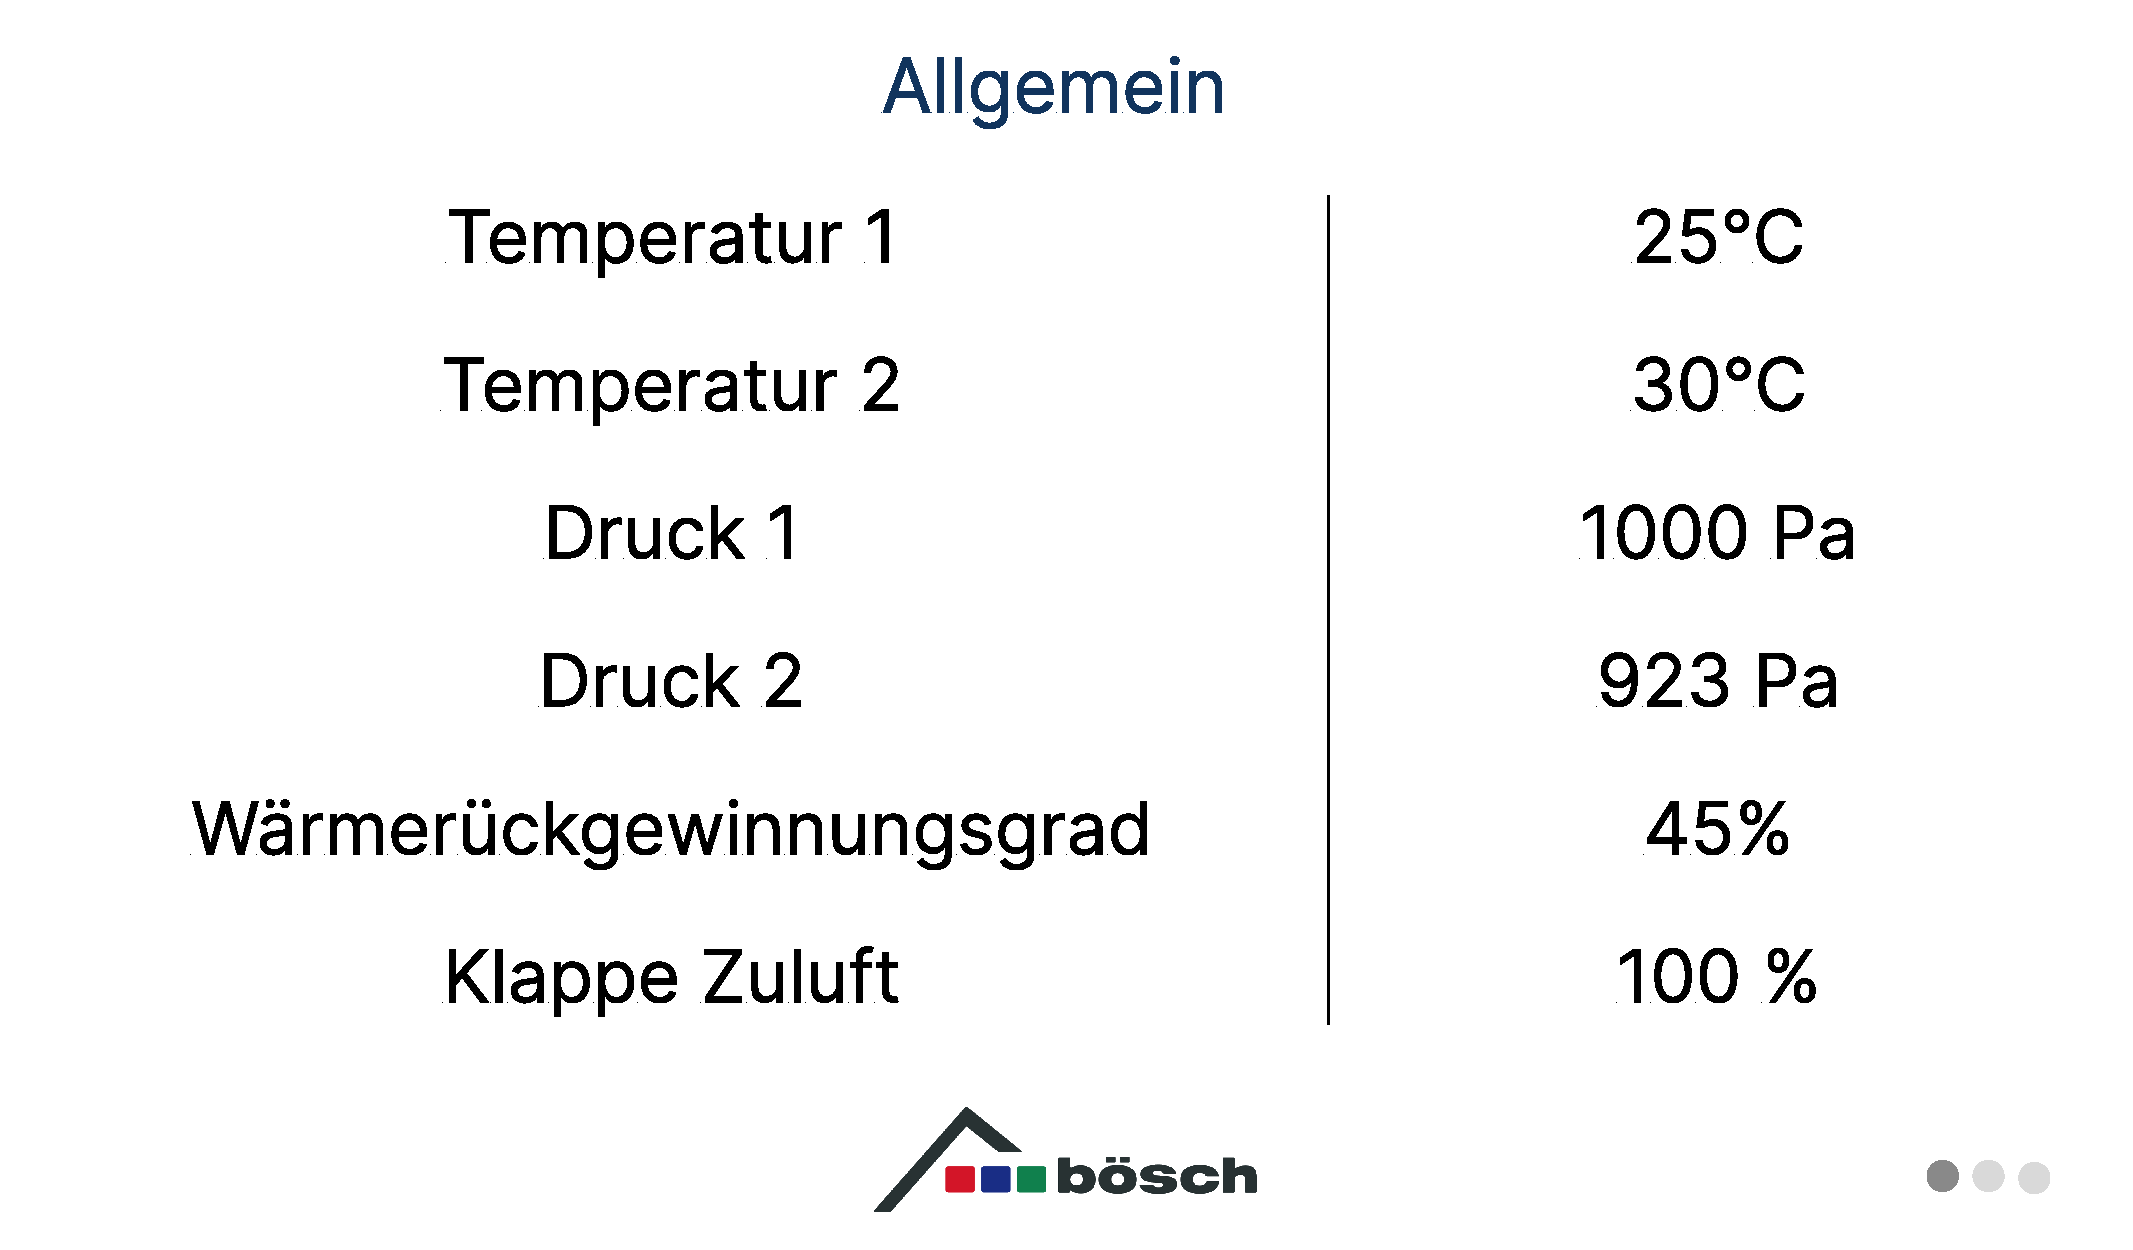
\includegraphics[width=0.99\textwidth, page=1]{design_varianten}}
    		\caption{Design Variante A \label{fig:variante_a}}
    	\end{subfigure}
        \hfill
    	\begin{subfigure}[t]{0.49\textwidth}
    		\centering
    		\frame{\includegraphics[width=0.99\textwidth, page=2]{design_varianten}}
    		\caption{Design Variante B \label{fig:variante_b}}
    	\end{subfigure}
    \begin{subfigure}[t]{\textwidth}
		\centering
		\frame{\includegraphics[width=0.70\textwidth, page=3]{design_varianten}}
		\caption{Design Variante C \label{fig:variante_c}}
	\end{subfigure}
	\caption{\acs{gui} Design Varianten \label{fig:design_varianten}}
\end{figure}

Mit den zuletzt genannten Kriterien wurden drei Designvarianten entworfen (siehe Abb. \ref{fig:design_varianten}). Zur Umsetzung gelangte schlussendlich Variante C (siehe Abb. \ref{fig:variante_c}). Diese bietet mit dem Kontrast im Hintergrund jedes einzelnen Messwerts und der listenartigen Aufzählung die besten Eigenschaften, um Messwerte auf einem Display mit begrenzter Auflösung und Helligkeit in Umgebungen mit suboptimalen Bedingungen ablesen zu können. 


\subsection{Umsetzung der GUI im Code}\label{tkintercode}
\paragraph{Klassenstruktur}
Im Vordergrund basiert die Klassenstruktur grundsätzlich auf \gls{gls_ctk} Komponenten (siehe Abb.~\ref{fig:klassenstruktur_frontend}). Dabei gibt es die Klassen \lstinline{App}, \lstinline{PageFrame}, \lstinline{TitleFrame} und \lstinline{MeasurementFrame}. Im Programm wird eine \lstinline{App} Instanz ausgeführt, welche das Hauptfenster ist. Diese Instanz kann beliebig viele \lstinline{PageFrames} enthalten, die wiederum jeweils ein \lstinline{TitleFrame} und eine Liste von \lstinline{MeasurementFrames} beinhalten. Die \lstinline{PageFrames} stellen die einzelnen Seiten dar, welche per Knopfdruck an der \acs{rltanzeige} durchgeblättert werden können. In einem \lstinline{TitleFrame} wird immer der Titel der jeweiligen Seite gespeichert \bzw angezeigt. In den \lstinline{MeasurementFrame} Instanzen werden hingegen die tatsächlichen Messwerte (Bezeichnung + Wert + Maßeinheit) dargestellt.

\begin{figure}[H]
	\centering
	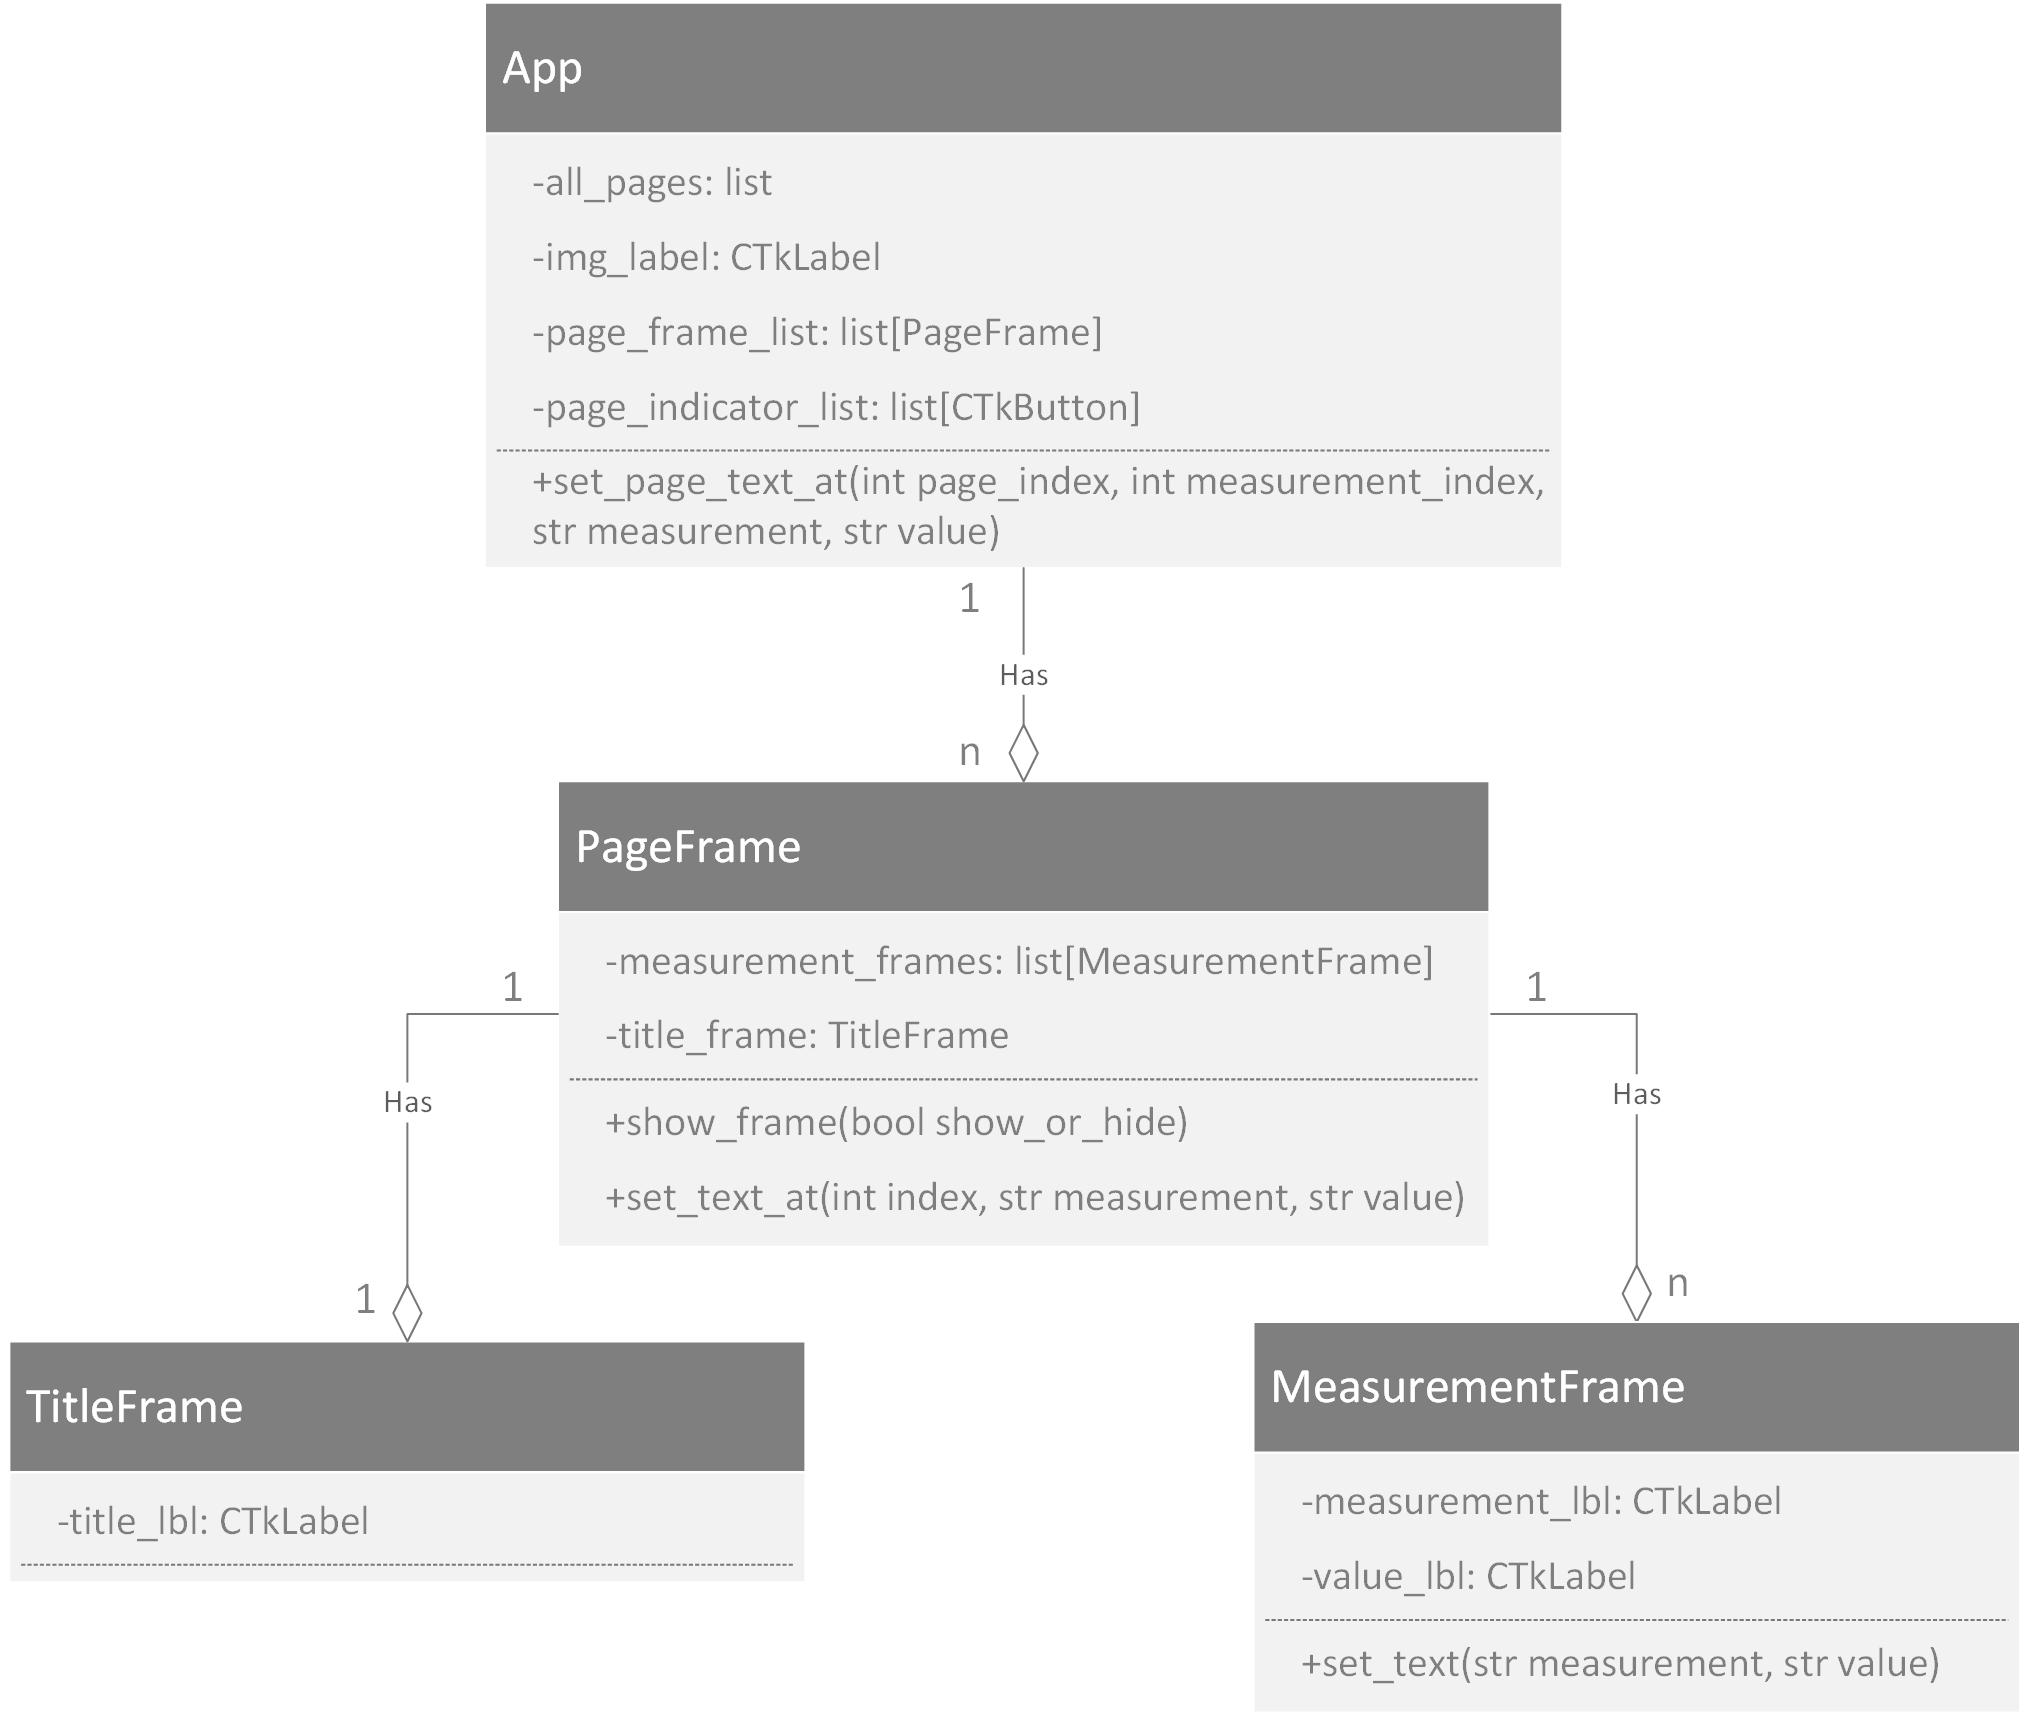
\includegraphics[width=0.95\textwidth]{uml_frontent_class_diagram}
	\caption{UML Diagramm Frontend \label{fig:klassenstruktur_frontend}}
\end{figure}

\paragraph{CustomTkinter Code}

Eine nähere Beschreibung und die Umsetzung der vorher genannten Klassen erfolgt in diesem Kapitel. 
\newline Wie zuletzt beschrieben, basieren alle Klassen im Frontend auf \gls{gls_ctk}. Die Klassen sind dabei alle (bis auf die Klasse \lstinline{App}) vom Typ \lstinline{CTkFrame}. Ein \lstinline{CTkFrame} ist ein Widget, das wie ein Rahmen \bzw Behälter für andere Widgets fungiert. So können diese in weiteren Widgets gruppiert und besser organisiert werden. Als erster Parameter wird für \lstinline{CTkFrames}, wie bei allen \gls{gls_tk} und \gls{gls_ctk} Widgets, der \lstinline{master} \bzw das Elternobjekt angegeben. Darüber hinaus können die Breite (\lstinline{width}), Höhe (\lstinline{height}), Rahmenbreite \bzw -Farbe (\lstinline{border_width} \bzw \lstinline{border_color}) sowie die Hintergrundfarbe (\lstinline{fg_color}) angegeben werden. \cite[vgl.][]{Schimansky:o.J.}

Die Klasse \lstinline{TitleFrame} enthält ein \lstinline{CTkLabel}, welches mit der \lstinline{place()} Methode im Behälter platziert wird. Die Klasse \lstinline{CTkLabel} basiert auf der Klasse \lstinline{tkinter.Label} und dient zur Darstellung eines Textes. Im \lstinline{TitleFrame} Label steht immer der Titel der zugehörigen Seite. Das \lstinline{title_font} Objekt, welches im folgenden Code zu sehen ist, ist eine Instanz der \gls{gls_ctk} Utility Klasse \lstinline{CTkFont}. Es wird verwendet, um die Schriftformatierung von \gls{gls_ctk} Widgets vorzunehmen. Jedes \gls{gls_ctk} Widget bekommt standardmäßig ein \lstinline{CTkFont} Objekt, wobei ein solches Objekt zeitgleich mehreren Widgets angefügt werden kann. Eine Änderung eines \lstinline{CTkFont} Objekts wird an alle Widgets, die es verwenden, weitergeleitet. \cite[vgl.][]{Schimansky:o.J.}

\begin{pythoncode}
class TitleFrame(ctk.CTkFrame):
	def __init__(self, master, title, **kwargs):
		super().__init__(master, width=800, height=60, fg_color=text_color, **kwargs)
		
		title_font = ctk.CTkFont(family="Roboto", size=32)
		
		self.title_lbl = ctk.CTkLabel(master=self, text=title, width=700, height=45, fg_color="transparent", text_color=title_color, anchor=ctk.CENTER, font=title_font)
		self.title_lbl.place(relx=0.5, rely=0.12, anchor=ctk.N)
\end{pythoncode}


Wie in der Klassenstruktur beschrieben, beinhaltet ein jedes \lstinline{PageFrame} neben einem \lstinline{TitleFrame} eine Liste von \lstinline{MeasurementFrames}. Eine Instanz der Klasse \lstinline{MeasurementFrame} enthält immer Informationen zu einem bestimmten Messwert, welche mithilfe von zwei \lstinline{CTkLabel} Widgets dargestellt werden. Dabei wird die Bezeichnung des Messwerts links im \lstinline{measurement_lbl} und der tatsächliche Wert einschließlich Maßeinheit rechts im \lstinline{value_lbl} platziert. Die zwei Labels werden durch einen Strich getrennt, der mit dem \gls{gls_tk} Widget \enquote{Canvas} erstellt wird. Ein Canvas ist ein rechteckiger Bereich \bzw eine Leinwand, auf dem Bilder oder andere komplexe Layouts gezeichnet werden können. Zusätzlich lassen sich auf einem Canvas Widget \zB weitere Widgets, Text oder Bilder platzieren. \cite[vgl.][20]{Shipman:2013} 
\newline Da jeder Messwert kontinuierlich aktualisiert wird, verfügt die \lstinline{MeasurementFrame} Klasse über die Methode \lstinline{set_text()}. In dieser wird mithilfe der \lstinline{configure()} Methode der Text beider Labels aktualisiert. Es folgt ein gekürzter Code zur \lstinline{MeasurementFrame} Klasse.

\begin{pythoncode}
class MeasurementFrame(ctk.CTkFrame):
	def __init__(self, master, measurement, value, **kwargs):
		#[Initialisierung des CTkFrames + Erstellung eines CTkFont Objekts zur Schriftformatierung der MeasurementFrames]
		
		self.measurement_lbl = ctk.CTkLabel(master=self, text=measurement, ...)
		self.value_lbl = ctk.CTkLabel(master=self, text=value, ...)
		self.canvas = Canvas(master=self, ...)
		#[Platzierung beider Labels + Canvas]
		
	def set_text(self, value):
		self.value_lbl.configure(text=value)
\end{pythoncode}

Die letzte der \gls{gls_ctk} \lstinline{CTkFrame} Klassen ist die \lstinline{PageFrame} Klasse. Wie bereits erwähnt ist jede Instanz dieser Klasse ein unsichtbarer Behälter, der ein \lstinline{TitleFrame} sowie eine Liste von \lstinline{MeasurementFrames} beinhält und als Seite dient. Diese Komponenten werden, wie im nachstehenden Code zu sehen ist, im Konstruktor eines jeden \lstinline{PageFrames} zugeordnet. Die Parameter \lstinline{title} und \lstinline{measurement} stammen aus der \acs{json} Haupt-Konfigurationsdatei (siehe Kapitel \ref{json_config_files}, Tab. \ref{tab:pages_array_parameter} unter \enquote{title} \bzw Tab. \ref{tab:sources_array_parameter}  unter \enquote{description}) und können daher schon bei Erstellung der \lstinline{PageFrame} Instanzen übergeben werden. Der \lstinline{value} Parameter der individuellen \lstinline{MeasurementFrames} hingegen wird laufend von der Methode \lstinline{set_text_at()} aktualisiert und ist daher am Anfang bis zum ersten Auslesen auf \enquote{N/A} (\dt nicht verfügbar) gesetzt.
	
\begin{pythoncode}
class PageFrame(ctk.CTkFrame):
	def __init__(self, master, title, parameters, **kwargs):
		#[Initialisierung des CTkFrames]
		self.measurement_frames = []
		self.title_frame = TitleFrame(master=master, title=title, ...)
		
		for parameter in parameters:
			frame = MeasurementFrame(master=master, measurement=parameter.description, value="N/A", ...)
			self.measurement_frames.append(frame)

    def set_text_at(self, index, value):
        self.measurement_frames[index].set_text(value)
...
\end{pythoncode}

Die \lstinline{PageFrame} Klasse enthält zudem eine \lstinline{show_frame()} Methode, die dazu dient die jeweilige \lstinline{PageFrame} Instanz \bzw ihren Inhalt sichtbar oder unsichtbar zu machen. Diese Methode ist notwendig, um zwischen den unterschiedlichen Seiten wechseln zu können \bzw die Seitenstruktur (siehe Kapitel \ref{figma_design}) für die jeweilige \acs{rltanzeige} umzusetzen.

\begin{pythoncode}
...
	def show_frame(self, show_or_hide):
		if show_or_hide:
			self.title_frame.place(...)
			self.title_frame.tkraise()
		else:
			self.title_frame.place_forget()
		
		for my_frame in self.measurement_frames:
			if show_or_hide:
				my_frame.place(...)
				my_frame.tkraise()
			else:
				my_frame.place_forget()
\end{pythoncode}

Die Klasse \lstinline{App} ist eine Instanz der \gls{gls_ctk} Window Klasse \lstinline{CTk}. Die \lstinline{CTk} Klasse bildet als Hauptfenster die Grundlage für jedes \gls{gls_ctk} Programm. Dabei sollte während der Laufzeit eines Programmes immer nur eine Instanz der \lstinline{CTk} Klasse existieren, wobei weitere Fenster mit der \lstinline{CTkToplevel} Klasse erstellt werden können. Mit Aufruf der \lstinline{mainloop()} Methode wird das Programm gestartet.
\cite[vgl.][]{Schimansky:o.J.} 

Folgend ist ein vereinfachter Code des Konstruktors der Klasse \lstinline{App} zu sehen. Hier wird das Hauptfenster aufgesetzt. Dabei wird zuerst mit den Methoden \lstinline{attributes()}, \lstinline{resizable()} und \lstinline{config()} die Größe des Fensters festgelegt, sowie der Cursor deaktiviert, da die \acs{rltanzeige} durch Taster gesteuert wird und dieser daher irrelevant ist. Daraufhin wird das Logo der Firma Bösch hinzugefügt. Dafür kommt die \gls{gls_ctk} Utility Klasse \lstinline{CTkImage} zum Einsatz, die als Behälter für das Bild dient und wiederum mithilfe eines \lstinline{CTkLabels} im Hauptfenster platziert wird.

\begin{pythoncode}
class App(ctk.CTk):
	def __init__(self, all_pages, page_frame_list, page_indicator_list, *args, **kwargs):
		super().__init__(*args, **kwargs)
		self.attributes('-fullscreen', True)
		self.resizable(False, False)
		self.config(cursor="none")
		
		boesch_logo = ctk.CTkImage(light_image=Image.open("..."), dark_image=Image.open("..."), size=(x, y))
		self.img_label = ctk.CTkLabel(master=self, image=boesch_logo, text="")
		self.img_label.place(...)
...
\end{pythoncode}

% Weiters werden im Konstruktor die globalen Listen \enquote{page\_frame\_list } und \enquote{page\_indicator\_list} erstellt, die zur Verwaltung der \enquote{PageFrames} sowie Indikatoren für die Seitenanzeige dienen.

Weiters wird im Konstruktor für jede Seite in der Liste \lstinline{all\_pages} ein \lstinline{PageFrame} erstellt und der \lstinline{page_frame_list} hinzugefügt. Die Liste \lstinline{all_pages} ist eine Liste mit allen nötigen Informationen für ein \lstinline{PageFrame} und wird im Backend des Programmes erstellt (siehe Kapitel \ref{auslesen_rlt_parameter}). Die \lstinline{page_frame_list} ist eine globale Liste, die zur Verwaltung der \lstinline{PageFrames} dient. Anschließend wird das erste \lstinline{PageFrame} sichtbar gemacht, indem die Methode \lstinline{show_frame(True)} aufgerufen wird.
%\lstinline{show_frame(True)}

\begin{pythoncode}
...	
		for page in all_pages:
			page_frame_list.append(PageFrame(master=self, title=page.title, parameters=page.measurements))
   
		page_frame_list[0].show_frame(True)
...
\end{pythoncode}

Zuletzt werden im Konstruktor die Seitenindikatoren erstellt und platziert. Jeder Indikator wird mithilfe des \gls{gls_ctk} Widgets \lstinline{CTkButton} erstellt und ist somit grundsätzlich ein grauer, runder Knopf ohne Text. Mithilfe der globalen Variable \lstinline{current_page} wird dabei erkannt, ob die zum Knopf zugehörige Seite angezeigt wird und daraus abgeleitet, ob dieser Hellgrau oder Dunkelgrau erstellt werden soll.

Die Position der Seitenindikatoren wird basierend auf der Anzahl der Seiten dynamisch berechnet. Wenn mehr als eine Seite vorhanden ist, wird für jede Seite in der Liste \lstinline{page_frame_list} ein Indikator erstellt und platziert, wie im folgenden Code vereinfacht gezeigt wird.

\begin{pythoncode}
...
		if len(page_frame_list) > 1:
			for i in range(0, len(page_frame_list)):
				page_indicator_list.append(ctk.CTkButton(master=self, ..., fg_color=("hellgrau" if i == current_page else "dunkelgrau")))
				page_indicator_list[i].place(relx=start_x_position + number,...)
...
\end{pythoncode}

Die Klasse \lstinline{App} beinhaltet eine Methode mit dem Namen \lstinline{set_page_text_at()}. Sie wird in der \lstinline{data_refresh()} Methode aufgerufen (siehe Kapitel \ref{auslesen_rlt_parameter}), welche dazu dient, die Messwerte regelmäßig zu aktualisieren.

\begin{pythoncode}
	def set_page_text_at(self, page_index, measurement_index, value):
    	page_frame_list[page_index].set_text_at(measurement_index, value)
\end{pythoncode}

\paragraph{Code zur Navigation der Seiten mit GPIO Tastern}

Nachdem die Erstellung der einzelnen Seiten mittels \gls{gls_ctk} erfolgt ist, müssen Methoden definiert werden, um an der \acs{rltanzeige} mit zwei Tastern zwischen diesen Seiten wechseln zu können. Eine kurze Erklärung dieser Methoden erfolgt in diesem Kapitel.

Um auf die \ac{gpio} Pins des Raspberry PIs \bzw die Taster der \acs{rltanzeige} zugreifen zu können wird die \enquote{RPi.GPIO} Bibliothek verwendet, welche im untenstehenden Code als \lstinline{GPIO} importiert wurde. Das ganze geschieht in der Methode \lstinline{setup_buttons()}, die als Teil des Anfangs des Programms ausgeführt wird.
Als Erstes wird mit \lstinline{setmode(GPIO.BOARD)} angegeben, dass die pysikalischen Pinnummern des Raspberry PIs verwendet werden. Alternativ kann \lstinline{setmode(GPIO.BCM)} verwendet werden, um die logischen \ac{gpio} Pinnummern zu verwenden. Daraufhin wird jedem Taster ein \ac{gpio} Pin zugeordnet. Weiters werden für die beiden Taster entsprechende Ereignisdetektoren eingerichtet, die bei Betätigung der Taster die entsprechende Callback-Funktion (\lstinline{last_page()} \bzw \lstinline{next_page()}) aufrufen.

\begin{pythoncode}
def setup_buttons():
    last_page_button = #[Pinnummer des "Zurück"-Tasters]
    next_page_button = #[Pinnummer des "Weiter"-Tasters]

    GPIO.setmode(GPIO.BOARD)
    
    GPIO.setup(last_page_button, GPIO.IN, pull_up_down=GPIO.PUD_UP)
    GPIO.add_event_detect(last_page_button, GPIO.FALLING, callback=last_page, bouncetime=300)

    #[Gleiche Konfiguration für den anderen Taster. Der callback wird aber auf "next_page" gesetzt]
\end{pythoncode}

Die Funktion \lstinline{last_page()} wird aufgerufen, wenn der "Zurück"-Taster gedrückt wird. Zuerst wird überprüft, ob es mehr als eine Seite gibt, da sonst kein Wechseln auf eine andere Seite möglich wäre. Dann wird die globale Variable \lstinline{current_page} um eins verringert, um zur vorherigen Seite zu wechseln. Falls \lstinline{current_page} dabei negativ wird, wird \lstinline{current_page} auf den Index der letzten Seite gesetzt, um eine zyklische Navigation der Seiten zu ermöglichen. Anschließend werden sowohl  die Seiten an sich als auch die Farbe die Seitenindikatoren aktualisiert, um den aktuellen Stand zu reflektieren. Dabei werden zuerst alle Seiten \bzw \lstinline{PageFrames} ausgeblendet und daraufhin die aktuelle Seite wieder sichtbar gemacht. Auch bei den Seitenidentifikatoren werden zuerst alle hellgrau gemacht, bevor der zur aktuellen Seite zugehörige Indikator in einem dunkleren grau dargestellt wird.

\begin{pythoncode}
def last_page(channel):
    if len(page_frame_list) < 2:
        return

    globals_.current_page -= 1
    if current_page < 0:
        current_page = len(page_frame_list) - 1

    for f in page_frame_list:
        f.show_frame(False)
    page_frame_list[current_page].show_frame(True)  

    for i in range(0, len(page_frame_list)):
        page_indicator_list[i].configure(fg_color="hellgrau")
    page_indicator_list[current_page].configure(fg_color="dunkelgrau")
\end{pythoncode}

Die \lstinline{next_page()} Methode wird dann aufgerufen, wenn der "Weiter"-Taster gedrückt wird. Sie funktioniert ähnlich wie \lstinline{last_page()}, jedoch wird \lstinline{current_page} um eins erhöht, um zur nächsten Seite zu wechseln. Dazu wird \lstinline{current_page}, um eine zyklische Navigation zu ermöglichen, auf Null zurückgesetzt, wenn die Variable den Index der letzten Seite überschreitet.



\section{\acs{json} Konfigurationsdateien}
\setAuthor{\pezze}
Raumlufttechnische Anlagen beinhalten unterschiedlichste Komponenten, beispielsweise Ventilatoren, Luftdrucksensoren und Temperatursensoren, mit denen die Funktion überwacht und gesteuert wird. Weil die \acsp{rltanlage} der Firma Bösch auf Kundenanforderungen angepasst werden, ist die Anordnung und Menge der verbauten Komponenten in den meisten Fällen unterschiedlich. Daher ist es wichtig, dass die \acs{rltanzeige} parametrierbar ausgeführt werden kann. Um dies zu erzielen, wurde vom Projektauftraggeber die Idee einer Konfigurationsdatei vorgeschlagen. Mit dieser kann von einer  Servicetechnikerin \bzw einem Servicetechniker bei der Installation der \acs{rltanlage} die Konfiguration an die \acs{rltanzeige} übergeben werden. So können für die jeweilige \acs{rltanlage} immer die richtigen Parameter angezeigt werden.

Wegen der Tatsache, dass diese Konfigurationsdateien von Servicetechnikerinnen und Servicetechnikern erstellt werden müssen, ist es wichtig, dass das gewählte Datenformat für Laien einfach zu verstehen ist. Daher lag die Entscheidung für das richtige Datenformat zwischen \acs{csv} und \acs{json}. Andere Formate  wie \acf{xml} wurden nicht in Erwägung gezogen, weil das Projektteam mit \acs{json} und \acs{csv} schon vertraut war. Darüber hinaus ist \acs{xml} im Vergleich zu \acs{json} für Laien schwerer zu lesen und schreiben, was es für die Anwendung ungeeignet macht. 

\subsection{Was ist CSV?}\label{csv_kapitel}
\acf{csv} ist ein systemunabhängiges Format für Klartextdateien mit der Dateiendung \enquote{.csv}. \acs{csv} Dateien dienen zum Speichern und Übertragen von strukturierten Daten, hauptsächlich Tabellen oder Listen, wobei durch die Verkettung von mehreren \acs{csv} Dateien oder mithilfe von zusätzlichen Regeln auch verschachtelte Objekte gespeichert werden können. Die hauptsächlichen Anwendungsbereiche von \acs{csv} Dateien sind zum Importieren und Exportieren von Daten aus Datenbanken oder die Migration von Tabellendaten zwischen Programmen. \cite[vgl.][]{FuchsMediaSolutions:o.J.}

Die erste Verwendung des Datenformates geht auf 1972 zurück, wo es vom IBM FORTRAN IV (H Extended) Compiler unterstützt wurde. \cite[vgl.][]{IBM:1972} Trotz der langen Existenz gibt es gegenwärtig für \acs{csv} keine formelle Spezifikation. Mit dem \acs{rfc} 4180 \cite[vgl.][]{Shafranovich:2005} aus dem Jahre 2005 existiert ein erster Versuch einer inoffiziellen Definition, welche mittlerweile weit verbreitet ist. Durch dieses Dokument wird das \acf{mime} \enquote{text/csv} für das \acs{csv} Format registriert. Es folgen die wesentlichen Merkmale aus der Definition des \acs{rfc} 4180:

\begin{enumerate}{}
	
	\item Jedem Datensatz steht eine Zeile zu, die mit einem Zeilenumbruch (\ac{crlf}) beendet wird. Ein Zeilenumbruch am Ende des letzten Datensatzes ist optional. \zB 
	\begin{lstlisting}
	aaa, bbb, ccc CRLF
	xxx, yyy, zzz CRLF
	\end{lstlisting}
	oder
	\begin{lstlisting}
	aaa, bbb, ccc CRLF
	xxx, yyy, zzz
	\end{lstlisting}
	
	\item Am Anfang eines \acs{csv} Dokumentes kann es eine Kopfzeile geben. Diese hat das Format eines normalen Datensatzes und beinhaltet Namen für die Spalten (Felder). Die Anzahl der Spalten sollte für Kopfzeile und Datensätze gleich sein. \zB
	\begin{lstlisting}
	spaltenname_1, spaltenname_2, spaltenname_3 CRLF
	xxx, yyy, zzz CRLF
	\end{lstlisting} %	aaa, bbb, ccc CRLF
	
	\item Sowohl in den Datensätzen als auch in der Kopfzeile kann es eine oder mehrere Spalten geben, die jeweils immer durch einen Beistrich (\acs{engl} comma) separiert werden. Am Ende einer Zeile bedarf es keines Beistrichs. Abstände sind Teil eines Feldes und müssen berücksichtigt werden. (Anmerkung: Auch wenn das eigentliche Format Beistriche für die Feldtrennung vorsieht, werden oft andere Zeichen wie \zB Strichpunkte (Semikolons) verwendet.)
	
	\item Jedes Feld kann in Anführungszeichen eingeschlossen sein und darf dann auch Beistriche, Zeilenumbrüche oder Anführungszeichen beinhaltet. \zB
	\begin{lstlisting}
	"aaa","b CRLF
	bb","ccc" CRLF
	xxx,yyy,zzz
	\end{lstlisting}
	
\end{enumerate}

Da es bei \acs{csv} keine festen Vorgaben beim Datenformat gibt, ist es die Verantwortung der Benutzer sich auf eine Formatierung zu einigen. Das führt oft zu Problemen bei Zeit- und Datumsangaben oder bei der Verwendung von Sonderzeichen. Eine weitere Hürde ist die fehlende explizite Angabe des verwendeten Zeichensatzes, womit \zB Umlaute fehlerhaft dargestellt werden können. \cite[vgl.][]{FuchsMediaSolutions:o.J.}

\subsection{Was ist JSON?}\label{json_kapitel}
\begin{minipage}{0.6\textwidth}
	\acf{json} wurde 2001 auf der \enquote{JSON.org} Website veröffentlicht und ist ein ressourcenschonendes Textformat zum Speichern von strukturierten Daten. Es ist so konzipiert, dass es sowohl für Menschen einfach zu lesen und schreiben als auch für Maschinen einfach zu parsen und generieren ist. Die Dateiendung von \acs{json} Dateien ist \enquote{.json}. \acs{json} stammt von JavaScript, ist aber programmiersprachenunabhängig und folgt vielen Konventionen der C-basierten Sprachen, was es gut für den Datenaustausch macht. \cite[vgl.][]{json_org:o.J., ECMA:2017}
\end{minipage}%
\hfill
\begin{minipage}{0.37\textwidth}
	\centering	
	
\includegraphics[width=0.58\textwidth]{JSON_logo}
	\captionof{figure}{\acs{json} Logo (Quelle:\\
		 \url{https://en.m.wikipedia.org/wiki/File:JSON_vector_logo.svg}) \label{fig:json_logo}}
\end{minipage}
\vspace{1ex}

\acs{json} wird derzeit von zwei Spezifikation definiert, ECMA-404 \cite[vgl.][]{ECMA:2017} und RFC 8259 \cite[vgl.][]{Bray:2017}. Dabei unterscheidet sich nur die Beschreibung des Formats, die \acs{json} Syntax beider Spezifikationen ist ident. Folgend wird sich auf die Beschreibung der offiziellen JSON.org Website \cite[vgl.][]{json_org:o.J.} und somit auf ECMA-404 \cite[vgl.][]{ECMA:2017} bezogen.

Die zwei wichtigsten Strukturen auf denen \acs{json} aufbaut sind Name/Wert (\engl Key/Value) Paare und geordnete Listen von Werten. Dabei unterstützt \acs{json} sehr verschachtelte Strukturen. Um diese darzustellen, werden in der Syntax folgende Zeichen benötigt:
\begin{itemize}
	 \item Beistriche \lstinline|,|
	 \item Doppelpunkte \lstinline|:|
	 \item Eckige Klammern \lstinline|[ ]|
	 \item Geschwungene Klammern \lstinline|{ }|
\end{itemize}


Mithilfe dieser Syntax, kann man in \acs{json} folgende Strukturen umsetzen:
\begin{itemize}
	\item \textbf{Values} (\dt Werte) sind, entweder vom Typ \enquote{object}, \enquote{string}, \enquote{array}, \enquote{number} oder haben den Wert \enquote{false}, \enquote{true}, oder \enquote{null} (siehe Abb.~\ref{fig:json_value}).
	\begin{figure}[H]
		\centering
		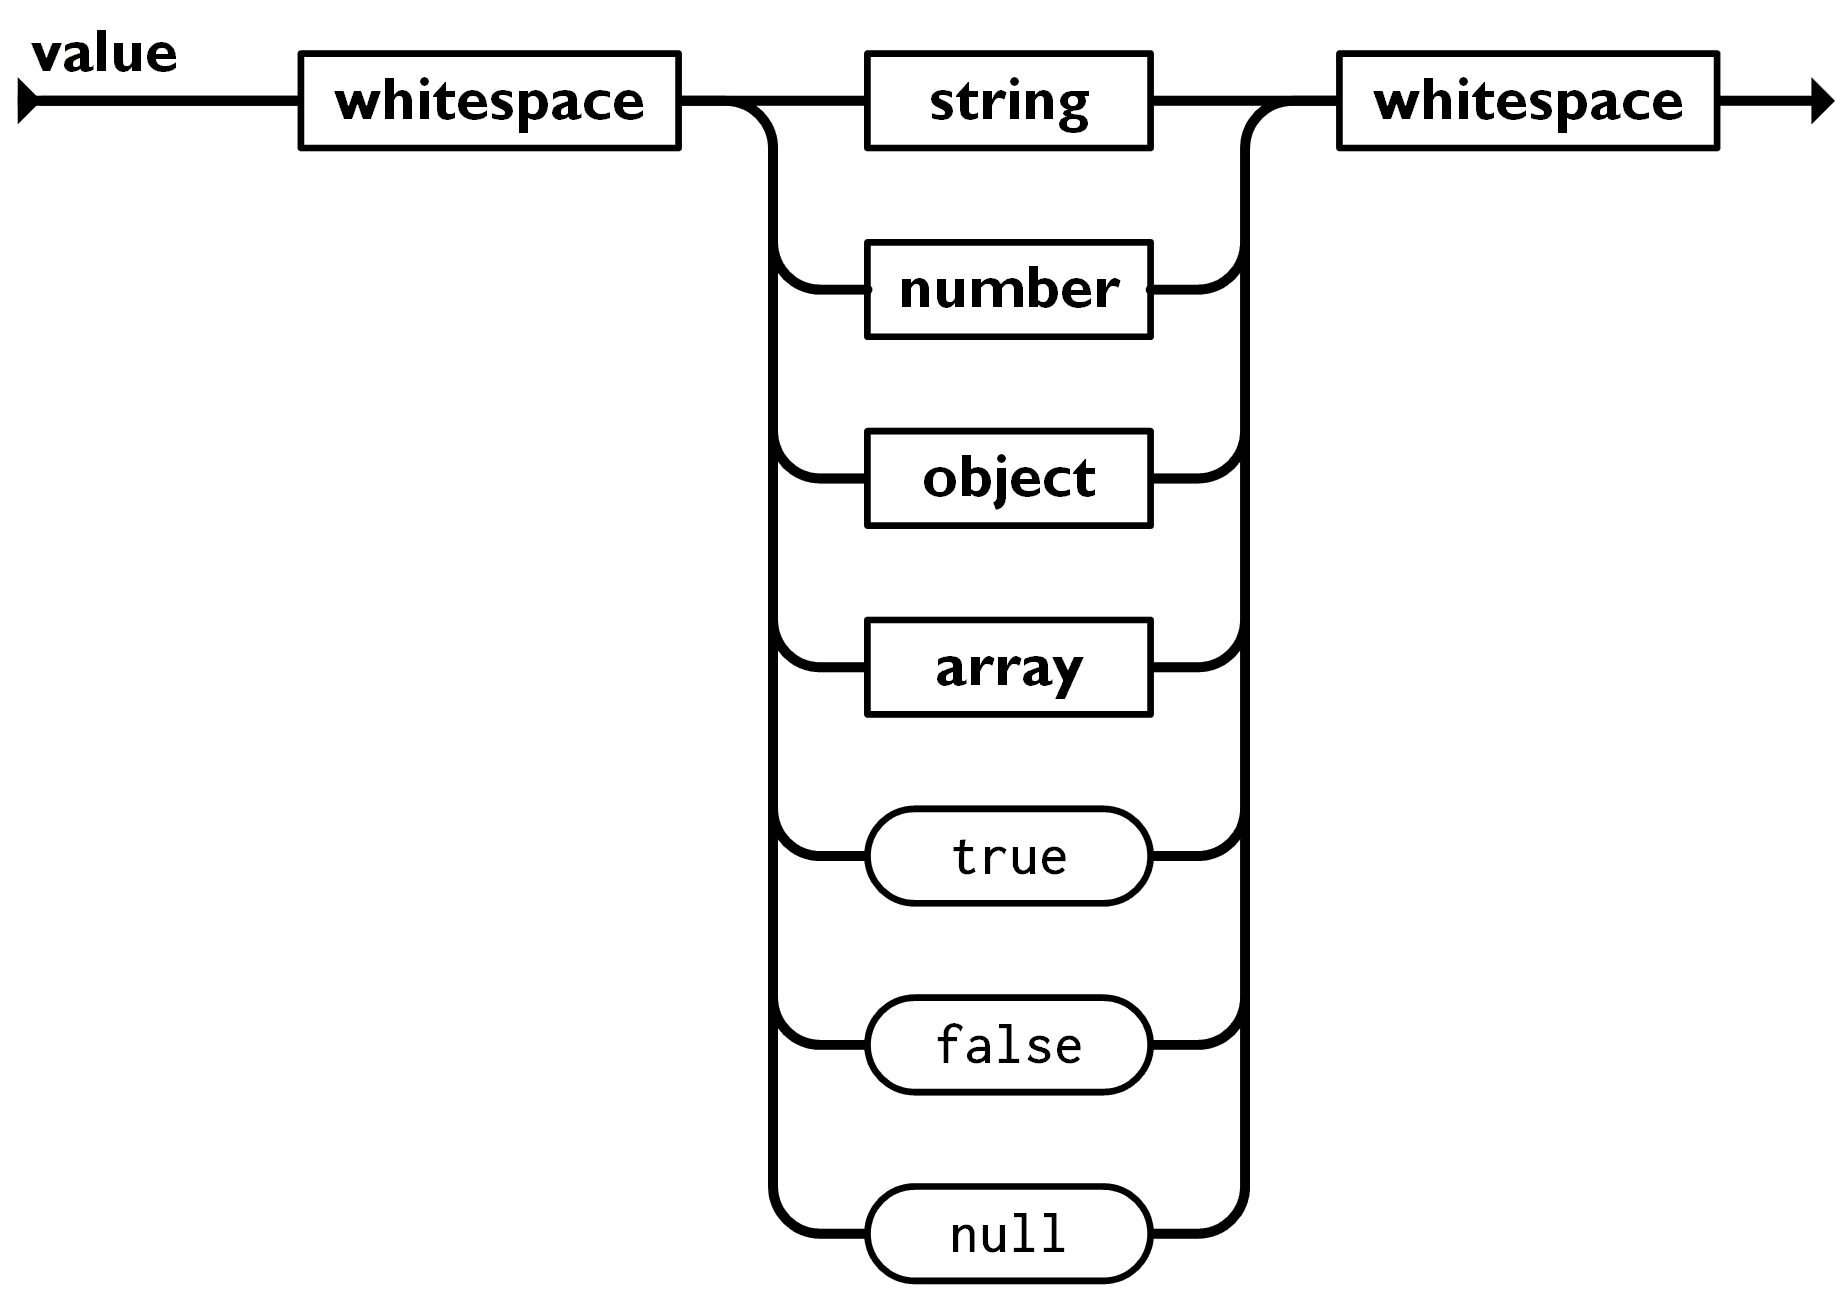
\includegraphics[width=10cm]{JSON_value}
		\caption{\acs{json} Value (Quelle: \url{https://www.json.org/img/value.png})  \label{fig:json_value}}
	\end{figure}
	
	\item \textbf{Objects} (\dt Objekte) sind ungeordnete Listen von beliebig vielen Name/Wert Paaren. Ein Name/Wert Paar besteht immer aus einem Namen, gefolgt von einem Doppelpunkt und dem zugehörigen Wert. Beistriche kommen zum Einsatz um Name/Wert Paare voneinander zu trennen. Ein Objekt wird immer von geschwungenen Klammern umschlossen. Der Aufbau eines \acs{json} Objekts ist in Abb.~\ref{fig:json_object} zu sehen.
	
	\begin{figure}[H]
		\centering
		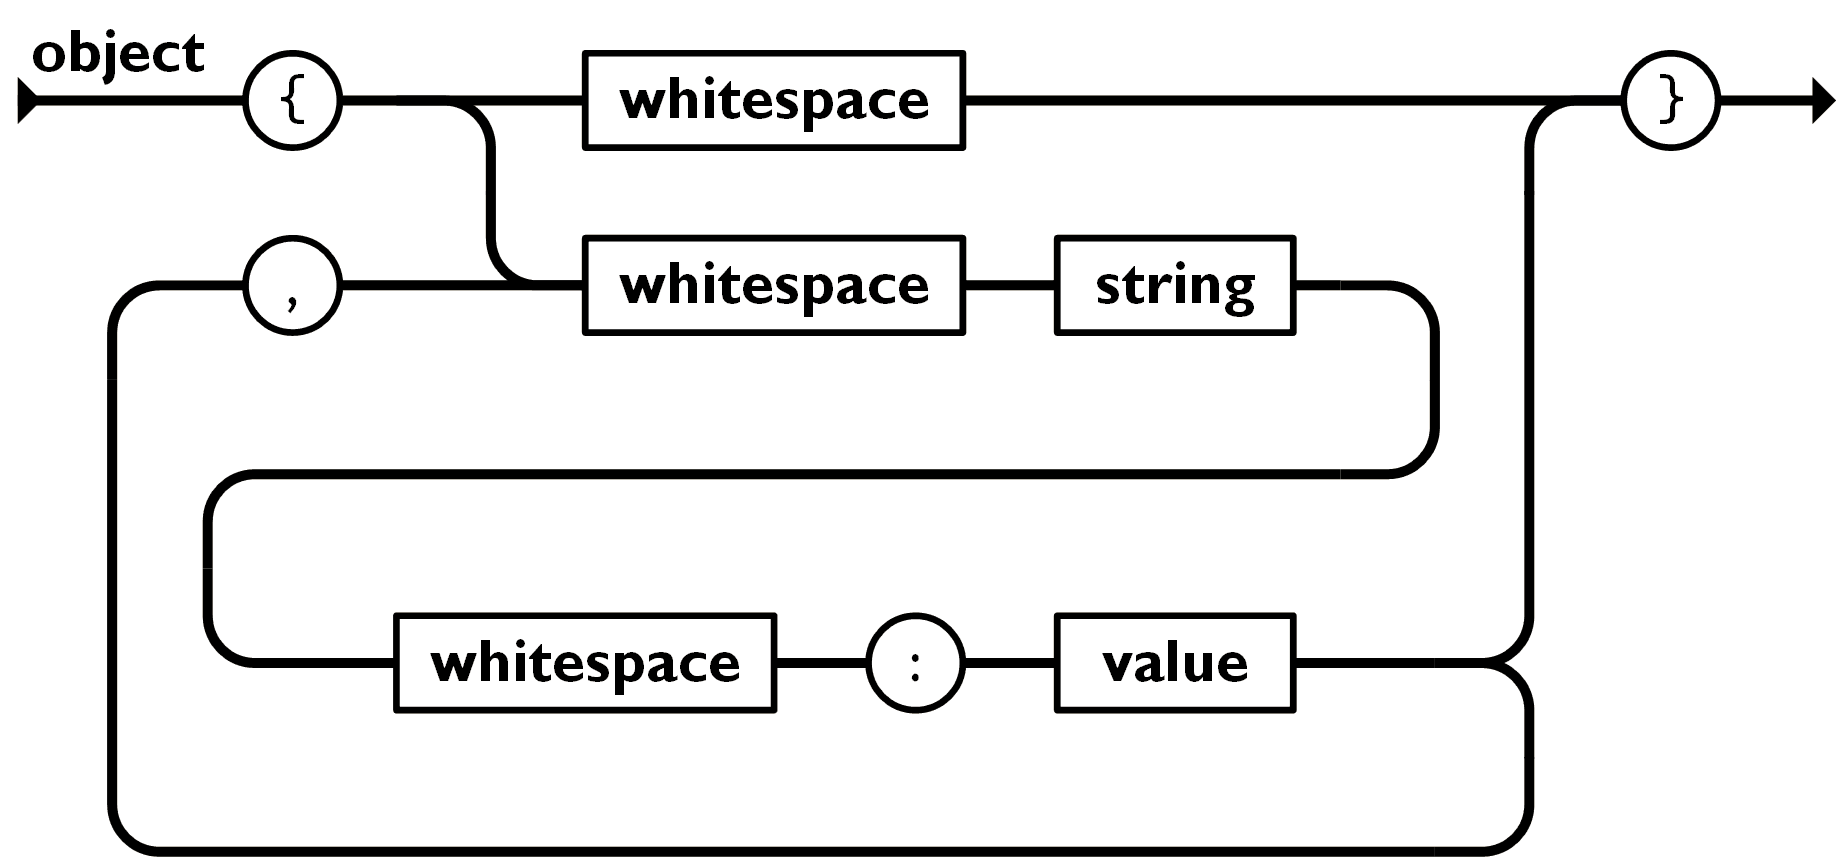
\includegraphics[width=10cm]{JSON_object}
		\caption{\acs{json} Object (Quelle: \url{https://www.json.org/img/object.png})  \label{fig:json_object}}
	\end{figure}
	
	\item \textbf{Arrays} sind geordnete Listen von Werten. Dabei werden Beistriche verwendet, um die Werte voneinander zu trennen. Ein Array wird immer von eckigen Klammern umschlossen. Der Aufbau eines Arrays ist in Abb.~\ref{fig:json_array} zu sehen.
	
	\begin{figure}[H]
		\centering
		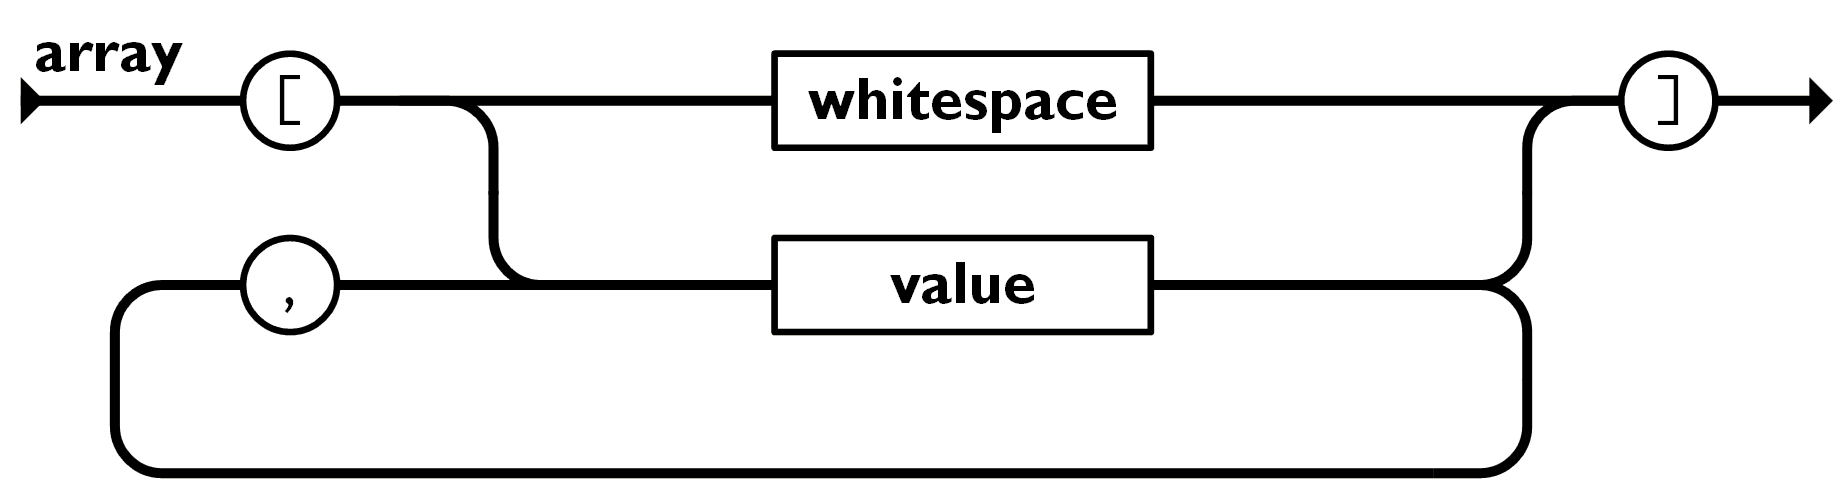
\includegraphics[width=10cm]{JSON_array}
		\caption{\acs{json} Array (Quelle: \url{https://www.json.org/img/array.png})  \label{fig:json_array}}
	\end{figure}
	
	\item \textbf{Strings} sind Zeichenketten. Sie können entweder leer sein, d. h. aus keinen Zeichen bestehen oder mehrere Unicode Zeichen enthalten. Eine Zeichenkette wird immer von Anführungszeichen umschlossen. Sie kann auch besondere Escapesequenzen beinhalten, die besondere Bedeutungen haben. Diese werden mit einem Backslash aufgerufen, wie \zB \enquote{\textbackslash n}, \enquote{\textbackslash t} oder \enquote{\textbackslash r}.
	
	\item \textbf{Numbers} (\dt Zahlen) sind numerische Werte, die aus einer oder mehreren dezimalen Ziffern bestehen. Sie können also keine Werte wie \zB \enquote{Infinity} oder \enquote{NaN} annehmen. Außerdem werden sie nie von Anführungszeichen umschlossen. 
	
\end{itemize}

Beispiele für \acs{json} Dateien sind in Kapitel \ref{json_config_files} zu finden.

\subsection{\acs{json} und \acs{csv} - Vergleich und Selektion} \label{json_vs_csv}
Sowohl \acs{json} als auch \acs{csv} bringen Vorteile mit sich. 
\acs{csv} Dateien können in Microsoft Excel bearbeitet und erstellt werden. Die tabellarische Darstellung und die Bekanntheit von Excel machen es zugänglich für Laien, was der größte Vorteil für \acs{csv} ist. Außerdem wird \acs{csv} von vielen Programmiersprachen unterstützt, was die Umsetzung theoretisch möglich machen würde. 

\acs{json} Dateien sind hingegen \acs{csv} zwar für Laien schwererer zu lesen, bieten aber hinsichtlich meist anderer Aspekte deutlich mehr Möglichkeiten. Anstatt des tabellarischen Aufbaus wird zum Speichern der Daten eine klare hierarchische Struktur verwendet. Die Struktur sorgt für mehr Flexibilität und eine besonders gute Darstellung verschachtelter Daten. Auch unterstützt \acs{json} unterschiedliche Datentypen, während bei \acs{csv} grundsätzlich nur Zeichenketten zum Einsatz kommen.

\acs{json} ist mittlerweile an Kompatibilität kaum zu übertreffen, was dessen Verwendung unbedenklich macht. Das Datenformat wird in unzähligen Bereichen eingesetzt und der Trend scheint immer weiter gegen \acs{json} zu gehen.

Schließlich überwiegen, im benötigten Anwendungsbereich, die vielen Vorteile von \acs{json} die schlechtere Leserlichkeit. Vor allem war die Möglichkeit der Verschachtelung der ausschlaggebende Grund weshalb sich für das \acs{json} Datenformat entschieden wurde. Dazu ist es wahrscheinlich, dass, wegen ihrem logischen Aufbau und  Skalierbarkeit, \acs{json} Dateien für den Anwendungszweck im Endeffekt übersichtlicher als \acs{csv} Dateien sind.

Falls bei Einführung der \acs{rltanzeige} Schwierigkeiten mit der Konfiguration auftreten steht \zB die Option eines Skripts, welches Excel Dateien in das gewünschte \acs{json} Format übersetzt, zur Verfügung.


\subsection{Dateikonzept} \label{json_config_files}
Für das Dateikonzept wurden drei Dateitypen auf Basis von \acs{json} Dateien entwickelt. Abbildung \ref{fig:vereinfachter_aufbau_dateikonzept} dient dem besseren Verständnis des Dateikonzepts. Hauptsächlich zeigt diese einen vereinfachten Aufbau der Komponenten, die von der Firma Bösch zur Entwicklung einer \acs{rltanzeige} bereitgestellt wurden, und die dazugehörigen Konfigurationsdateien. Die \acs{rltanzeige} selbst ist über den Bus mit einem Ventilator von ebm-papst sowie einem QBM9711 von Siemens verbunden. Der Ventilator verfügt lediglich über integrierte Sensorik. Der QBM9711 hingegen verfügt über zwei integrierte Luftdruck-Sensoren (interne Ports 1 und 2), zwei (an die Ports Analog Input 1 und 2) extern angeschlossene Temperatursensoren, eine (an den Port Analog Output 1) extern angeschlossene Klappe und ein (an den Port Analog Output 2) extern angeschlossenes Relais.


\begin{figure}[H]
	\centering
	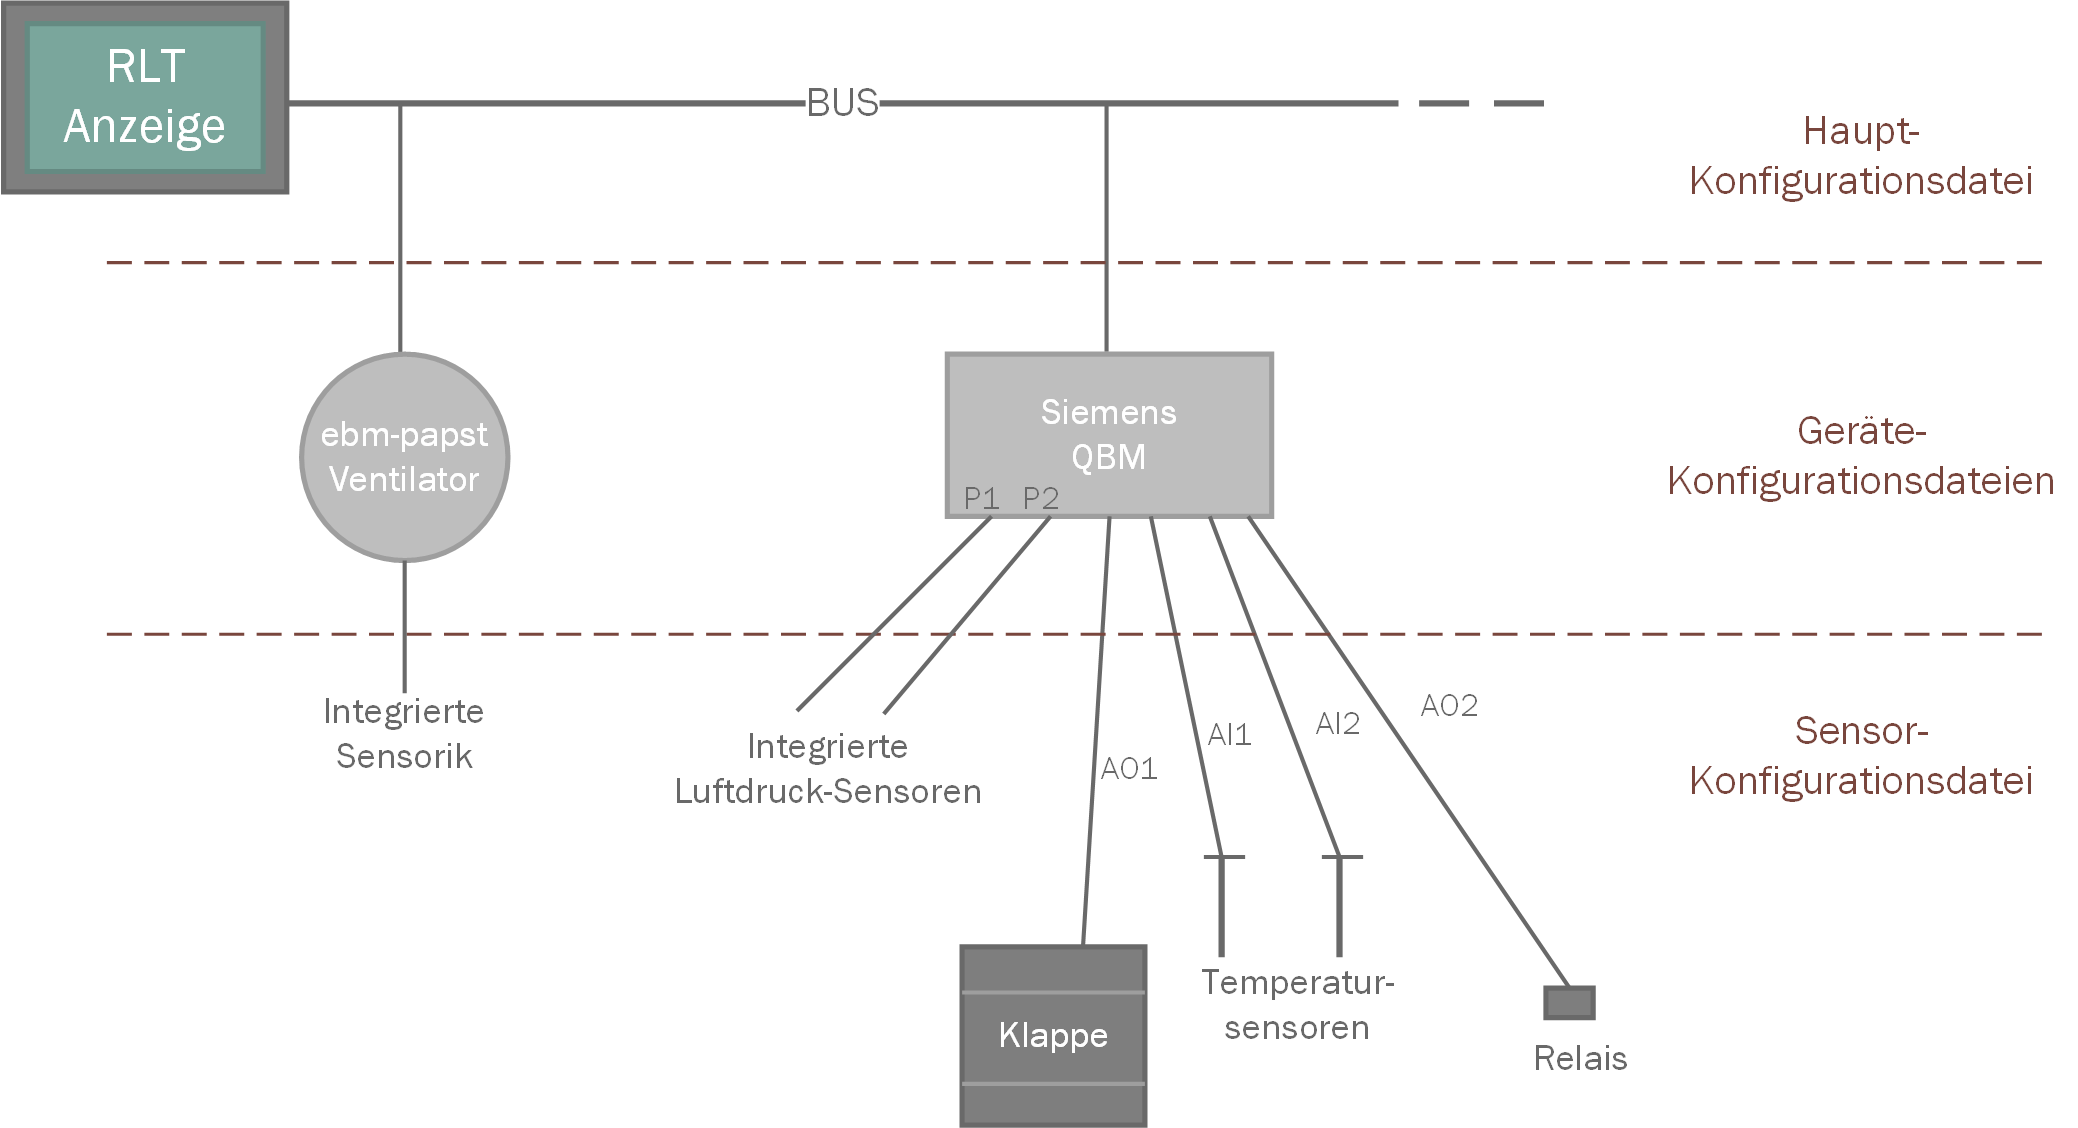
\includegraphics[width=\textwidth]{Komponenten_simpler_Aufbau_fuer_Dateikonzept}
	\caption{Vereinfachter Aufbau der Komponenten \label{fig:vereinfachter_aufbau_dateikonzept}}
\end{figure}

Es folgt eine aufbauende Beschreibung und Erklärung der drei Dateitypen:
%Fenkart fragen, ob ich bei den Geräten auf seinen Teil verweisen kann
% Wer beschreibt baud_rate, register, adresse, function code \ref{modbus_funktionsweise}

\begin{enumerate}

	\item \textbf{Sensor-Konfigurationsdatei} (\enquote{sensors.json}): Es gibt kein explizites Modbus Register, um die Maßeinheit eines Messwerts zu übertragen. Deswegen muss die Maßeinheit der unterschiedlichen Sensorik aus Datenblättern entnommen und jeweils zugeordnet werden. Dazu dient die Sensor-Konfigurationsdatei, welche eine Liste aller Sensoren (\zB bestimmte Temperatursensoren) mit der jeweils dazugehörigen Maßeinheit beinhaltet. Komponenten wie Ventilatoren haben integrierte Sensoren. Auch in diesem Fall kann für die Maßeinheit ein Eintrag in die \enquote{sensors.json} Datei gemacht werden. 
	
	Die einfache Ergänzung neuer Sensoren ist der Zweck der Sensor-Konfigurationsdatei. Diese muss nur dann verändert werden, wenn ein neuer Sensortyp, der noch nicht in der Sensor-Konfigurationsdatei steht, ergänzt wird. 
	
	Jeder Eintrag der Sensor-Konfigurationsdatei hat zwei Parameter, welche in Tab. \ref{tab:sensors_json_parameter} zu sehen sind.
		
	\begin{table}[h]
		\caption{Parameter der Sensor-Konfigurationsdatei (\enquote{sensors.json})}
		\label{tab:sensors_json_parameter}
		\begin{tabular}{p{\dimexpr 0.15\textwidth-2\tabcolsep} p{0.5\textwidth} | p{0.3\textwidth}}
			\toprule
			\textbf{Name} & \textbf{Beschreibung} & \textbf{Beispiel} \\
			\midrule
			type & Der Sensorname, auf den später in der Haupt-Konfigurationsdatei unter \enquote{type} referenziert wird. &  
			\begin{jsonTable}
"type": "NI1000"
			\end{jsonTable} 
 			\\
			unit & Die Einheit des entsprechenden Sensors. (Diese muss auch in der Geräte-Konfigurationsdatei unter \enquote{units} vorhanden sein.) &  
			\begin{jsonTable}
"unit": "°C"
			\end{jsonTable} 
			\\
			\bottomrule
		\end{tabular}
	\end{table}
	
		
	\item \textbf{Geräte-Konfigurationsdateien} (\zB \enquote{QBM97XX.json} oder \enquote{EBM.json}): Hier sind gerätespezifische Daten hinterlegt. Hauptsächlich welche Ausgabeports eine bestimmte Komponente (\zB ein Ventilator) besitzt, welche Einstellungen diese Ausgänge haben und \ggf welche Maßeinheiten die integrierten oder extern angeschlossenen Sensoren zurückgeben. 
	
	Weil in den \acs{rltanlagen} der Firma Bösch häufig die gleichen Komponenten verwendet werden, wurden spezielle Geräte-Konfigurationsdateien konzipiert. Diese Dateien können in der Haupt-Konfigurationsdatei beliebig oft referenziert werden, da sie einmalig für jedes Gerätemodell erstellt werden und nur selten Änderungen unterliegen. Das Hinzufügen einer neuen Geräte-Konfigurationsdatei ermöglicht zudem die einfache Integration einer neuen Komponente, beispielsweise eines Ventilators einer anderen Marke.
	
	Der Aufbau der Geräte-Konfigurationsdateien basiert auf einem \enquote{ports} Array. In dieses werden mithilfe der Parameter aus Tabelle \ref{tab:ports_array_parameter} die erforderlichen Informationen eingetragen.
	
	\begin{table}[H]
		\caption{Parameter des \enquote{ports} Array der Geräte-Konfigurationsdateien}
		\label{tab:ports_array_parameter}
		\begin{tabular}{p{\dimexpr 0.18\textwidth-2\tabcolsep} p{0.5\textwidth} | p{0.27\textwidth}}
			\toprule
			\textbf{Name} & \textbf{Beschreibung} & \textbf{Beispiel} \\
			\midrule
			port      	& Bezeichnung des Ausgabeports. Wird im Falle eines Geräts mit externer Sensorik (\zB Siemens QBM) in der Haupt-Konfigurationsdatei unter \enquote{port} referenziert. & 
			\begin{jsonTable}
"port": "AI1"
			\end{jsonTable} 
			\\
			register 	& Modbus Register (Erklärung in Kapitel \ref{modbus_funktionsweise}) in dem der jeweilige Messwert gespeichert ist \bzw welches ausgelesen werden soll. Das Register muss dabei immer dezimal angegeben werden, da minimalmodbus die hexadezimale Eingabe nicht unterstützt. & 
			\begin{jsonTable}
"register": 11
			\end{jsonTable} 
			\\
			function\_code 	& Modbus Function Code (Erklärung in Kapitel \ref{modbus_funktionsweise}), mit dem auf das vorher angegebene Register zugegriffen werden soll. Die zwei meist verwendeten Function Codes sind \enquote{3} für Input Register und \enquote{4} für Holding Register. & 
			\begin{jsonTable}
"function_code": 3
			\end{jsonTable} 
			\\
			units 	& Array in dem jeder möglichen Maßeinheit für den jeweiligen Ausgabeport eine Skalierung zugeordnet wird. Die Skalierung dient \zB dazu, dem Messwert die angemessene Anzahl von Dezimalstellen zuzuweisen, da diese über Modbus nicht übertragen werden (Funktionsweise in Kapitel \ref{auslesen_rlt_parameter} erklärt).
			
			Wird bei Ports weggelassen, deren Werte nur von Python Funktionen (Erklärung in Kapitel \ref{python_functions}) zur Weiterverarbeitung verwendet werden.
			
			Die Parameter eines Objekts dieses Arrays sind in Tabelle \ref{tab:units_array_parameter} zu sehen.  & 
			\begin{jsonTable}
"units": "[ ]"
			\end{jsonTable} 
			\\
			\bottomrule
		\end{tabular}
	\end{table}
	
	
	
	\begin{table}[H]
		\caption{Parameter des Unterarray \enquote{units}}
		\label{tab:units_array_parameter}
		\begin{tabular}{p{\dimexpr 0.18\textwidth-2\tabcolsep} p{0.47\textwidth} | p{0.3\textwidth}}
			\toprule
			\textbf{Name} & \textbf{Beschreibung} & \textbf{Beispiel} \\
			\midrule
			unit      	& Die Maßeinheit, die aus der Sensor-Konfigurationsdatei referenziert wird. & 
			\begin{jsonTable}
"unit": "°C"
			\end{jsonTable} 
			\\
			scaling 	& Skalierung des Messwertes. Kann aus Datenblättern entnommen werden. & 
			\begin{jsonTable}
"scaling": 0.1
			\end{jsonTable} 
			\\
			\bottomrule
		\end{tabular}
	\end{table}
		
	\item \textbf{Haupt-Konfigurationsdatei} (\enquote{main\_config\_file.json}):
	Wie in Kapitel \ref{gui_design} beschrieben, ist zur übersichtlichen Darstellung der Messwerte eine Aufteilung in mehrere Abschnitte bzw. Seiten erforderlich. Auf diesen Seiten werden jeweils sinngemäß Messwerte zusammengefasst. Die Konfiguration der Seiten erfolgt in der Haupt-Konfigurationsdatei mithilfe von zwei parallelen Arrays: dem \enquote{pages}-Array und dem \enquote{devices}-Array. 	
	
	Im \enquote{devices} Array werden die alle Komponenten \bzw Quellen der \acs{rltanlage}, nämlich Ventilatoren und QBMs (vgl. Abb. \ref{fig:vereinfachter_aufbau_dateikonzept}), aufgeführt, von denen Messwerte ausgelesen werden sollen. Die Parameter des \enquote{devices} Arrays sind in Tabelle \ref{tab:devices_array_parameter} näher erläutert.
	
	\begin{table}[H]
		\caption{Parameter des \enquote{devices} Array der Haupt-Konfigurationsdatei}
		\label{tab:devices_array_parameter}
		\begin{tabular}{p{\dimexpr 0.17\textwidth-2\tabcolsep} p{0.48\textwidth} | p{0.3\textwidth}}
			\toprule
			\textbf{Name} & \textbf{Beschreibung} & \textbf{Beispiel} \\
			\midrule
			device     	& Angabe des Gerätetyps, indem auf den Namen der zugehörigen Geräte-Konfigurationsdatei referenziert wird. & 	
			\begin{jsonTable}
"device": "QBM97XX"
			\end{jsonTable}  
			\\
			id         	& Beliebig auswählbare, jedoch eindeutige Bezeichnung für das Gerät. Mit der \enquote{id} wird im \enquote{pages} Array auf das Gerät referenziert.  & 	
			\begin{jsonTable}
"id": "QBM1"
			\end{jsonTable}  
			\\
			baud\_rate	& Eingestellte Baudrate. Ist bei allen Komponenten einer \acs{rltanlage} gleich. & 	
			\begin{jsonTable}
"baud_rate": 19200
			\end{jsonTable}  
			\\
			mbaddress	& Die Modbus Adresse des Geräts. (vgl. Kapitel \ref{modbus_funktionsweise}) & 	
			\begin{jsonTable}
"mbaddress": 1
			\end{jsonTable}  
			\\
			parity	& Parität. Mögliche Werte: \enquote{even}, \enquote{odd} oder \enquote{none} (vgl. Kapitel \ref{modbus_uebertragungsarten}) & 	
			\begin{jsonTable}
"parity": "even"
			\end{jsonTable}  
			\\
			stop\_bits	& Anzahl der Stopbits einer Nachricht (vgl. Kapitel \ref{modbus_uebertragungsarten}) & 	
			\begin{jsonTable}
"stop_bits": 1
			\end{jsonTable}  
			\\
			zero\_based	& Gibt an, ob die Modbus Register von 0 oder 1 ausgehend gezählt werden. Mögliche Werte: \enquote{true} oder \enquote{false}.
			
			(Bemerkung: Bei Siemens QBMs normalerweise \enquote{false}, bei ebm-papst Ventilatoren \enquote{true}) & 	
			\begin{jsonTable}
"zero_based": false
			\end{jsonTable}  
			\\
			sensors	& Array aller am Gerät angeschlossenen Sensoren. Bei Ventilatoren und Ausgabeports, deren Werte ausschließlich von Python Funktionen zur Weiterverarbeitung genutzt werden (Erklärung in Kapitel \ref{python_functions}), wird auf die Angabe verzichtet. 
			
			Die zwei Parameter, die für jedes Objekt dieses Arrays angegeben werden, sind in Tabelle \ref{tab:sensors_array_parameter} zu finden. & 	
			\begin{jsonTable}
"sensors": [ ]
			\end{jsonTable}  
			\\
			\bottomrule
		\end{tabular}
	\end{table} 
	
	\begin{table}[H]
		\caption{Parameter des Unterarray \enquote{sensors}}
		\label{tab:sensors_array_parameter}
		\begin{tabular}{p{\dimexpr 0.18\textwidth-2\tabcolsep} p{0.45\textwidth} | p{0.32\textwidth}}
			\toprule
			\textbf{Name} & \textbf{Beschreibung} & \textbf{Beispiel} \\
			\midrule
			port   	& Verweist auf den Ausgabeport aus der Geräte-Konfigurationsdatei (siehe Tab. \ref{tab:ports_array_parameter}). Mögliche Werte können also \zB der Datei \enquote{QBM97XX.json} entnommen werden. & 	
			\begin{jsonTable}
"port": "AI1"
			\end{jsonTable}  
			\\
			type 	& Verweist auf einen Sensor aus der Sensor-Konfigurationsdatei. Mögliche Werte können also \zB der Datei \enquote{sensors.json} entnommen werden. & 	
			\begin{jsonTable}
"type": "LG-NI1000"
			\end{jsonTable}  
			\\
			\bottomrule
		\end{tabular}
	\end{table}
	

	Im \enquote{pages} Array werden alle Seiten, die später auf der \acs{rltanzeige} veranschaulicht werden sollen, definiert. Dabei werden die in Tabelle \ref{tab:devices_array_parameter} definierten Quellen den richtigen Seiten zugeordnet. Die Parameter des \enquote{pages} Array sind in Tabelle \ref{tab:pages_array_parameter} notiert.
	
	% unterschiedliche anzahl der Komponenten

	\begin{table}[H]
		\caption{Parameter des \enquote{pages} Array der Haupt-Konfigurationsdatei}
		\label{tab:pages_array_parameter}
			\begin{tabular}{p{\dimexpr 0.15\textwidth-2\tabcolsep} p{0.45\textwidth} | p{0.35\textwidth}}
			\toprule
			\textbf{Name} & \textbf{Beschreibung} & \textbf{Beispiel} \\
			\midrule
			title      	& Beliebig auswählbarer Titel der Seite. & 
			\begin{jsonTable}
"title": "Allgemein"
			\end{jsonTable} 
			\\
			sources 	& Array aller Messwerte, die auf einer Seite angezeigt werden sollen. Die Parameter, die in einem Objekt dieses Arrays benutzt werden, sind in Tab. \ref{tab:sources_array_parameter} zu sehen. & 
			\begin{jsonTable}
"sources": "[ ]"
			\end{jsonTable} 
			\\
			\bottomrule
		\end{tabular}
	\end{table}
	
	\begin{table}[H]
		\caption{Parameter des Unterarray \enquote{sources}}
		\label{tab:sources_array_parameter}
			\begin{tabular}{p{\dimexpr 0.2\textwidth-2\tabcolsep} p{0.42\textwidth} | p{0.33\textwidth}}
			\toprule
			\textbf{Name} & \textbf{Beschreibung} & \textbf{Beispiel} \\
			\midrule
			port                & Ein Array mit den Quellen, aus denen der Messwert ausgelesen wird. Dabei wird meistens nur ein Objekt mit \enquote{id} (siehe Tab. \ref{tab:devices_array_parameter}) des Geräts und \enquote{port} (siehe Tab. \ref{tab:ports_array_parameter}) angegeben. In einigen Szenarien ist es erforderlich, mehrere Quellen für abgeleitete Messwerte zu verwenden (siehe Kapitel \ref{python_functions}). In solchen Fällen werden dem Array zusätzliche Objekte hinzugefügt. &  
			\begin{jsonTable}
"port": [
	{ "QBM1": "AI1" }
]
			\end{jsonTable} 
			\\
			description         & Beliebig auswählbare Bezeichnung für den Messwert. Der Messwert wird später auf der \acs{rltanzeige} so bezeichnet. & 
			\begin{jsonTable}
"description": "Temperatur Zuluft"
			\end{jsonTable}  
			\\
			python\_function    & (Optionaler) Parameter, der nur angegeben wird, wenn der jeweilige Messwert abgeleitet berechnet werden muss. (Erklärung in Kapitel \ref{python_functions}). & 
			\begin{jsonTable}
"python_function": "relay_position"
			\end{jsonTable} 
			\\
			additional\_info    & (Optionaler) Parameter, der nur angegeben wird, falls die jeweilige Python Funktion zusätzliche Informationen benötigt. (Erklärung in Kapitel \ref{python_functions}). & 
			\begin{jsonTable}
"additional_info": { "switching_voltage": 5 }
			\end{jsonTable} 
			\\
			\bottomrule
		\end{tabular}
	\end{table} 
					
\end{enumerate}

%Bedienungsanleitung für Servicetechniker erwähnen
Zuletzt ist zu erwähnen, dass Servicetechnikerinnen und Servicetechniker zur Installation einen Ordner bekommen. Darin befindet sich direkt eine Vorlage für die \enquote{main\_config\_file.json} Datei, welche im Normalfall die einzige Datei sein sollte, die bearbeitet bzw. verändert wird.
In einem Unterordner (\enquote{devices}) sind Geräte-Konfigurationsdateien und die Sensor-Konfigurationsdatei zu finden. Diese Dateien müssen, wie gerade erwähnt, nur verändert werden, wenn noch nie verwendete Komponenten, wie z.B. eine neue Art von Ventilator oder Sensor, in der \acs{rltanlage} verbaut werden.

Ein Beispiel zu allen Dateitypen ist im Anhang zu finden.






\setAuthor{\schneider}
\subsection{Einlesen der Konfigurationsdateien} \label{einlesen_konfigurationsdateien}
\paragraph{Klassenstruktur}
Im Backend wird die Klassenstruktur der \ac{gui} nachgebildet. Es gibt eine \lstinline{Page}, eine \lstinline{Measurement} und eine \lstinline{Sensor} Klasse. Eine \lstinline{Measurement} Instanz kann mehrere \lstinline{Sensor} Instanzen enthalten, da manche \lstinline{Measurements} zur Berechnung (z.B. der Wärmerückgewinnungsgrad) mehrere Messwerte benötigen. Die \lstinline{Page} Instanzen speichern die jeweiligen \lstinline{Measurement} Instanzen, die auf dieser Seite angezeigt werden sollen. Die \lstinline{Page} Instanzen existieren, damit der ausgelesene Parameter an der richtigen Stelle auf der \acs{gui} verändert werden kann. Es gibt nämlich gleich viele \lstinline{Page} Instanzen wie \lstinline{PageFrame} Instanzen (vgl. Kapitel \ref{tkintercode}) und gleich viele \lstinline{Measurement} Instanzen wie \lstinline{MeasurementFrame} Instanzen. (siehe Abb.~\ref{fig:uml_backend}).
\begin{figure}[ht]
	\centering
	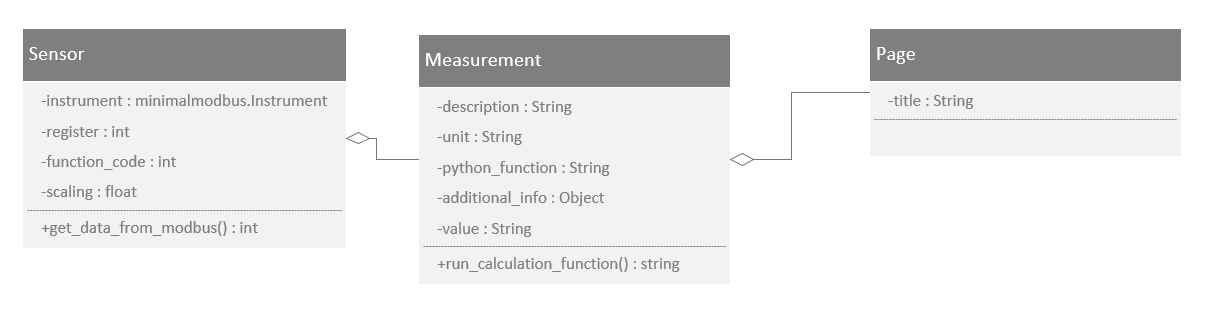
\includegraphics[width=1.0\linewidth]{Bilder/UML_Backend}
	\caption{UML Diagramm Backend}
	\label{fig:uml_backend}
\end{figure}

Die \lstinline{Page}, \lstinline{Measurement} und \lstinline{Sensor} Instanzen werden beim Einlesen der \acs{json} Konfigurationsdateien aufgrund der Objekte im \enquote{pages}  Array (vgl. Kapitel \ref{json_config_files}) erstellt und in Listen gespeichert. \newline
Zum Einlesen werden drei Funktionen implementiert:
\begin{itemize}
	\item \textbf{\lstinline{load_config()}:} Diese Funktion lädt die gesamte Haupt-Konfigurationsdatei ein. Es werden die angeschlossenen Geräte ermittelt und die \lstinline{Page}, \lstinline{Measurement} und \lstinline{Sensor} Instanzen erstellt. Dafür kommen die beiden folgenden Hilfsfunktionen zum Einsatz.
    \begin{itemize}
		\item \textbf{\lstinline{get_sensor_unit()}:} Liest die Sensor-Konfigurationsdateien ein. Dadurch können den Messwerten die richtigen Maßeinheiten zugewiesen werden.
		\item \textbf{\lstinline{get_sensor_data()}:} Liest aus der Geräte-Konfigurationsdatei am angegebenen Port die Parameter aus und liefert diese Parameter als \acs{json} Objekt zurück. Sie liest das Register, den \gls{modbus} Function Code und die Skalierung aus. Die Skalierung wird anhand der Maßeinheit aus der Sensor-Konfigurationsdatei ausgewählt.
	\end{itemize}
\end{itemize}

\paragraph{Einlesen und Erstellen der Instanzen}
Einlesen kann man ein \acs{json} Attribut mit folgender Syntax. Im folgenden Beispiel wird aus der Instanz namens \lstinline{page} das Attribut \enquote{title} gesucht und zurückgeliefert.
\begin{pythoncode}
title = page["title"]
\end{pythoncode}

Im folgenden Code werden die \lstinline{Measurement} Instanzen erstellt, indem die anzuzeigenden Messwerte aus dem \enquote{sources} Array iteriert werden. Anhand der Informationen der Objekte im \enquote{sources} Array werden dann die entsprechenden Geräte im \enquote{devices} Array herausgesucht. Es werden weitere Parameter aus der Haupt-Konfigurationsdatei ausgelesen, die zu dem entsprechenden Messwert gehören (z.B. die Bezeichnung oder die Einheit). Anschließend werden die \lstinline{Sensor} Instanzen erstellt und einer Liste beigefügt, da manche Measurements (z.B. die Rückwärmzahl) mehrere Messwerte benötigen. Diese Liste, sowie die vorher ausgelesenen Parameter werden beim Erstellen der \lstinline{Measurement} Instanzen dem Konstruktor übergeben und darin in Instanzvariablen gespeichert.
\begin{pythoncode}
page_measurements = []
for measurements in page["sources"]:
	measurements_sensors = []
	#[Auslesen weiterer Parameter der Haupt-Konfigurationsdatei (description, unit, python_function,additional_info)]
	#[Erstellen der Sensor Instanzen (Siehe nächster Codeblock)]
	page_measurements.append(Measurement(description=description, unit=unit, sensors=measurements_sensors, python_function=python_function, additional_info=additional_info))
\end{pythoncode}

Im folgenden Code wird für jeden Port (an jedem Port ist ein \lstinline{Sensor} angeschlossen) eines Geräts eine \lstinline{Sensor} Instanz erstellt. Alle \lstinline{Sensor} Instanzen werden der \lstinline{page_sensors} Liste beigefügt. Dafür gibt es im \enquote{sources} Array die einzelnen Ports. Das sind Wertepaare, die jeweils aus Gerät und \lstinline{Sensor} bestehen (vgl. Kapitel \ref{json_config_files}). Mit diesen beiden Werten kann dann das entsprechende Gerät im \enquote{devices} Array gefunden werden und darin der entsprechende Port im \enquote{sensors} Array. Mit der \lstinline{get_sensor_unit()} Funktion wird die Einheit erhalten und mit der \lstinline{get_sensor_data()} Funktion weitere Sensordaten. Diese werden beim Erstellen der \lstinline{Sensor} Instanz dem Konstruktor übergeben.
\begin{pythoncode}
port_counter = 0
for port in port_arr:
	device_id = list(port.keys())[port_counter] # example: QBM1
	port_id = port[device_id]  # example: AI1
	port_counter += 1
	
	for device in config_full_data[0]["devices"]:
		if device["id"] == device_id:
			#[Aufruf der get_sensor_unit Funktion]
			#[Auslesen der Geräteparameter in der Haupt-Konfigurationsdatei (baud_rate, mbaddress etc.)]
			#[Aufruf der get_sensor_data Funktion]
			measurements_sensors.append(Sensor(baud_rate=device["baud_rate"], ..., register=register, zero_based=device["zero_based"]))
\end{pythoncode}

Die \lstinline{Measurement} Instanzen sind nach dem Erstellen alle in einer Liste gespeichert. Zum Schluss werden \lstinline{Page} Instanzen erstellt. Die \lstinline{Measurement} Liste wird so aufgeteilt, dass maximal 5 Measurements auf einer Seite sind. Anhand dieser \lstinline{Page}- und \lstinline{Measurement} Instanzen wird beim Erstellen der \acs{gui} die Anzahl an Seiten übernommen, der Seitentitel und die Beschreibungen der Messwerte gesetzt (siehe Kapitel \ref{gui_design}). 
\begin{pythoncode}
counter = 0
last_slice = 0
for measurement in page_measurements:
	counter += 1
	if ((counter % 5) == 0) or (counter == len(page_measurements)):
		all_pages.append(Page(title=title, measurements=page_measurements[last_slice:counter]))
		last_slice = counter
\end{pythoncode}

%\pythonfile[firstline=125, lastline=197]{Code/modbus.py}

Im Konstruktor der \lstinline{Page}, \lstinline{Measurement} und \lstinline{Sensor} Klasse werden die ausgelesenen Variablen in Instanzvariablen gespeichert.

\section{Python Funktionen}
\setAuthor{\pezze}
\label{python_functions}
Messwerte werden aus Modbus Registern der unterschiedlichen Komponenten einer \acs{rltanlage} bezogen.  Grundsätzlich wird jeder ausgelesene Wert direkt auf der \acs{rltanzeige} angezeigt, wobei Skalierung und Maßeinheit hinzugefügt werden. In einigen Fällen muss jedoch ein Wert aus mehreren Messwerten abgeleitet werden, eine spezielle Umrechnung oder Ähnliches erfolgen, bevor der Wert auf der \acs{rltanzeige} dargestellt werden kann. In einem solchen Fall wird in der Haupt-Konfigurationsdatei im \enquote{pages} Array (vgl. Kapitel \ref{json_config_files}) der Name einer Python Funktion angegeben, die ausgeführt werden muss, um den erwünschen Wert zu erhalten. 

Diese Python Funktionen sind in der Datei \enquote{modbus\_functions.py} definiert, was den folgenden Vorteil bietet: Ein einfaches Hinzufügen neuer Komponenten, deren Messwerte abgeleitet werden müssen, ohne dass der restliche Code verändert werden muss. Bei der Integration einer neuen Komponente werden lediglich die nötigen Funktionen in der \enquote{modbus\_functions.py} Datei hinzugefügt und diese folgend in der Haupt-Konfigurationsdatei referenziert. Dies ermöglicht eine flexible  Erweiterung des Systems.

Eine solche Python Funktion hat den folgenden grundlegenden Aufbau:
\begin{pythoncode}
def Funktionsname(sensors, additional_info):
	...	
	return Ergebnis
\end{pythoncode}

Jede Funktion erwartet die Übergabeparameter \enquote{sensors} und \enquote{addictional\_info}. \enquote{sensors} ist eine Liste, die Objekte der Klasse \enquote{Sensor} beinhaltet. Ein Objekt der Klasse \enquote{Sensor} wiederum enthält alle erforderlichen Informationen, um einen Wert aus einem Modbus Register auszulesen, wie es in Kapitel \ref{auslesen_rlt_parameter} beschrieben wird. \newline 
Der Parameter \enquote{additional\_info} ermöglicht die Übermittlung weiterer Informationen, falls diese bei der Berechnung oder Ableitung der Werte benötigt werden.

Im folgenden Abschnitt werden die bisher definierten Python Funktionen beschrieben, eine weitere Erklärung zum Ablauf bei der Ausführung der Python Funktionen ist in Kapitel \ref{auslesen_rlt_parameter} zu finden.


\paragraph{Funktion \enquote{standard}}
Diese Funktion wird standardmäßig ausgeführt, wenn in der Haupt-Konfigurationsdatei (vgl. Kapitel \ref{json_config_files}) der Parameter \enquote{python\_function} nicht angegeben wird \bzw keine besondere Python Funktion angegeben wird. Die \enquote{standard} Funktion wird daher als einzige dieser Funktionen nie direkt in der Haupt-Konfigurationsdatei referenziert.

Wie im unten stehenden Code zu sehen ist, wird bei dieser Funktion nichts berechnet. Es wird lediglich die \enquote{get\_data\_from\_modbus} Funktion der \enquote{Sensor} Instanz aufgerufen, welche den Messwert aus dem jeweiligen Modbus Register ausliest und zurück gibt (weitere Erklärung in Kapitel \ref{auslesen_rlt_parameter}).

\begin{pythoncode}
def standard(sensors, additional_info):
	return sensors[0].get_data_from_modbus()
\end{pythoncode}


\paragraph{Funktion \enquote{calc\_rpm}}
Wird verwendet, um bei ebm-papst Ventilatoren die Soll- \bzw Ist-Drehzahl zu ermitteln. Dabei werden, wie im folgenden Code zu sehen ist, zwei Register ausgelesen. Daraufhin wird das Verhältnis der jeweiligen Drehzahl zur maximalen Drehzahl des Ventilators berechnet, das Ergebnis gerundet und in Prozent zurückgegeben.

\begin{pythoncode}
def calc_rpm(sensors, additional_info):
	max_value = sensors[1].get_data_from_modbus()
	rpm_value = (sensors[0].get_data_from_modbus() / 64000) * max_value
	ratio = rpm_value / max_value * 100.0
	return str(round(ratio, 1)) + " %"
\end{pythoncode}

Die Gleichung \eqref{glg:drehzahl_berechnung} für die Berechnung des Wertes \enquote{rpm\_value} stammt aus dem Datenblatt für ebm-papst Ventilatoren \cite[vgl.][118,122]{ebmpapst:2020}: 
\begin{equation}
	\text{rpm\_value}\left[\frac{1}{min}\right] = \frac{\text{Datenbytes}}{64000} \cdot \text{max\_value} \left[\frac{1}{min}\right]
	\label{glg:drehzahl_berechnung}
\end{equation} 

Eine Angabe in der Haupt-Konfigurationsdatei sieht wie folgt aus. Dabei ist zu sehen, dass im \enquote{port} Array zuerst die Quelle der Ist- \bzw Soll-Drehzahl (\enquote{RPMreal} \bzw \enquote{RPMtarget})und als zweites die Quelle der maximalen Drehzahl (\enquote{RPMmax}). Es wird keine \enquote{additional\_info} angegeben.

\begin{jsoncode}
"sources": [
	{
		"port": [
			{"EBM1": "RPMreal"},
			{"EBM1": "RPMmax"}
		],
		"description": "Drehzahl Istwert",
		"python_function": "calc_rpm"
	},
	...
]
\end{jsoncode}



\paragraph{Funktion \enquote{calc\_power}}
Wird verwendet, um den Leistungsverbrauch von ebm-papst Ventilatoren zu ermitteln. Dabei werden, wie im folgenden Code zu sehen ist, drei Register ausgelesen und mit diesen der Leistungsverbrauch berechnet. Daraufhin wird das Ergebnis gerundet und mit der Maßeinheit \enquote{$W$} zurückgegeben.

\begin{pythoncode}
def calc_power(sensors, additional_info):
	byte_value = sensors[0].get_data_from_modbus()
	Uz_value = sensors[1].get_data_from_modbus() / 1000 * 20
	Iz_value = sensors[2].get_data_from_modbus() / 1000 * 2
	power = (byte_value / 65536) * Uz_value * Iz_value
	return str(round(power, 1)) + " W"
\end{pythoncode}

Für die Berechnung des aktuellen Leistungsverbrauchs wurden folgende Gleichungen \eqref{glg:calc_power} \eqref{glg:calc_uz} \eqref{glg:calc_iz} aus dem Datenblatt für ebm-papst Ventilatoren abgeleitet \cite[vgl.][95,126]{ebmpapst:2020}: 
\begin{equation}
	\text{Uz\_value} \left[V\right] = \frac{\text{byte\_value} * 20 \left[mV\right]}{1000}
	\label{glg:calc_uz}
\end{equation} 
\begin{equation}
	\text{Iz\_value} \left[A\right] = \frac{\text{byte\_value} * 2 \left[mA\right]}{1000}
	\label{glg:calc_iz}
\end{equation} 

\begin{equation}
	\text{power} \left[W\right] = \frac{\text{byte\_value}}{65536} \cdot \text{Uz\_value}  \left[V\right] \cdot \text{Iz\_value} \left[A\right]
	\label{glg:calc_power}
\end{equation} 

Eine Angabe in der Haupt-Konfigurationsdatei sieht wie folgt aus. Dabei ist zu sehen, dass im \enquote{port} Array zuerst die Quelle \enquote{Power}, als zweites die Quelle \enquote{Uz} und zuletzt die Quelle \enquote{Iz} eines ebm-papst Ventilators angegeben werden. Es wird keine \enquote{additional\_info} angegeben.

\begin{jsoncode}
"sources": [
	{
		"port": [
			{"EBM1": "Power"},
			{"EBM1": "Uz"},
			{"EBM1": "Iz"}
		],
		"description": "Leistung",
		"python_function": "calc_power"
	},
	...
]
\end{jsoncode}



\paragraph{Funktion \enquote{eng\_status}}
Wird verwendet, um bei ebm-papst Ventilatoren den Motorstatus \bzw aktuelle Fehlermeldungen zu ermitteln. Dabei wird, wie im folgenden Code zu sehen ist, ein Register ausgelesen, worin ein Statuscode enthalten ist. Daraufhin wird dieser Statuscode in eine binäre Zeichenkette konvertiert und seine einzelnen Bits analysiert. Falls ein Bit den Wert \enquote{1} hat, wird zur Zeichenkette \enquote{error\_string} der Fehlercode angehängt. Die Zeichenkette \enquote{error\_string} wird zuletzt zurückgegeben und kann mithilfe des Datenblatt für ebm-papst Ventilatoren \cite[vgl.][119]{ebmpapst:2020} entziffert werden. 

\begin{pythoncode}
def eng_status(sensors, additional_info):
	status = sensors[0].get_data_from_modbus()
	binary_status = bin(status)
	error_string = ""
	counter = 0
	for s in reversed(binary_status):
		counter += 1
		if s == "1":
			if counter == 1:
				error_string += "PHA "
			...
			elif counter == 13:
				error_string += "UzLow "
			else:
				error_string += "Unbekannter Fehler"
			
	if error_string == "":
		error_string = "Kein Fehler"
	
	return error_string
\end{pythoncode}

Eine Angabe in der Haupt-Konfigurationsdatei sieht wie folgt aus. Dabei ist zu sehen, dass im \enquote{port} Array nur die Quelle \enquote{EngStatus} angegeben wird. Es wird keine \enquote{additional\_info} angegeben.

\begin{jsoncode}
"sources": [
	{
		"port": [
			{"EBM1": "EngStatus"}
		],
		"description": "Motorstatus",
		"python_function": "eng_status"
	},
	...
]
\end{jsoncode}



\paragraph{Funktion \enquote{calc\_wrg}}
Wird verwendet, um die Rückwärmzahl einer \acs{rltanlage} zu ermitteln. Diese Zahl, auf die sich unternehmensintern bei Bösch als Wärmerückgewinnungsgrad bezogen wurde, ist ein Maß für die Effizienz der Wärmerückgewinnung. Sie zeigt an, wie viel Wärme aus der Abluft zurückgewonnen werden kann. Die Berechnung der Rückwärmzahl kann entweder auf die Temperatur der Abluft oder der Fortluft bezogen werden, wobei sich hier, wegen der verfügbaren Sensorik, für letztere entschieden wurde. \cite[vgl.][]{Klingenburg:o.J.}\\
Es folgt die Formel \eqref{glg:wrg_berechnung} zur Berechnung der Rückwärmzahl sowie ein Bild \ref{fig:waermetauscher_wrg} zur besseren Interpretation: 
\begin{equation}
	\text{Rückwärmzahl} = \frac{\text{Ablufttemperatur} - \text{Fortlufttemperatur}}{\text{Ablufttemperatur} - \text{Außenlufttemperatur}}
	\label{glg:wrg_berechnung}
\end{equation} 

\begin{figure}[H]
	\centering
	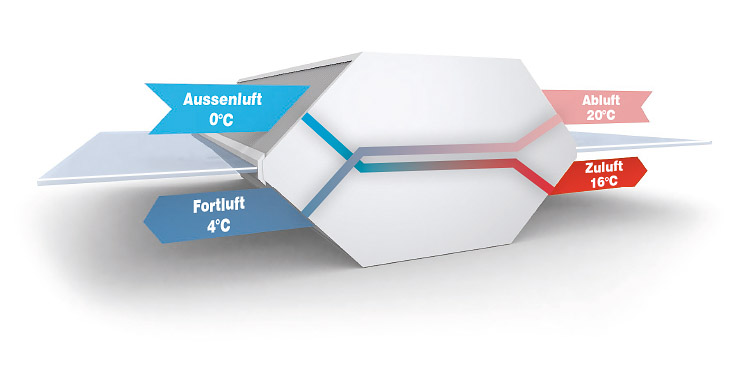
\includegraphics[width=0.7\linewidth]{Bilder/rueckwaermzahl_waermetauscher}
	\caption{Wärmetauscher mit unterschiedlichen Temperaturen (Quelle: \url{http://www.klingenburg.de/fileadmin/user_upload/germany/Wissen/rueckwaermzahlt_de_02.jpg})}
	\label{fig:waermetauscher_wrg}
\end{figure}
 
Die Umsetzung ist im folgenden Code zu sehen. Es werden die drei Temperaturwerte aus den jeweiligen Registern ausgelesen. Daraufhin wird der Wärmerückgewinnungsgrad berechnet, das Ergebnis gerundet und mit der Maßeinheit \enquote{\%} zurückgegeben.

\begin{pythoncode}
def calc_wrg(sensors, additional_info):
	exhaust_air = sensors[0].get_data_from_modbus()  # Abluft
	outgoing_air = sensors[1].get_data_from_modbus()  # Fortluft
	outside_air = sensors[2].get_data_from_modbus()  # Außenluft
	
	wrg = ((exhaust_air - outgoing_air) / (exhaust_air - outside_air)) * 100
	
	return str(round(wrg)) + " %"
\end{pythoncode}

Eine Angabe in der Haupt-Konfigurationsdatei sieht wie folgt aus. Dabei ist zu beachten, dass im \enquote{port} Array zuerst die Quelle der Ablufttemperatur, als zweites die Quelle der Fortlufttemperatur und zuletzt die Quelle der Außenlufttemperatur einer \acs{rltanlage} angegeben werden. Es wird keine \enquote{additional\_info} angegeben.

\begin{jsoncode}
	"sources": [
	{
		"port": [
			{"QBM2": "AI1"},
			{"QBM1": "AI2"},
			{"QBM1": "AI1"}
		],
		"description": "Wärmerückgewinnungsgrad",
		"python_function": "calc_wrg"
	},
	...
	]
\end{jsoncode}



\paragraph{Funktion \enquote{calc\_volume}}
Wird verwendet, um bei ebm-papst Ventilatoren den Volumenstrom zu ermitteln. Dieser gibt an, wie viel Luftvolumen der Ventilator pro Stunde befördert. Zur Bestimmung des Volumenstroms ($q_{V}$) kommt bei ebm-papst das Wirkdruckverfahren zum Einsatz, welches den statischen Druck vor und in der Einströmdüse vergleicht ($\rightarrow$ Differenzdruck der statischen Drücke $\Delta p$). \\
Die Formel für die Berechnung des Volumenstroms \eqref{glg:volumenstrom_berechnung} ist folgend zu sehen, wobei der K-Faktor \bzw Durchflussfaktor \cite[vgl.][]{rox_klimatechnik:o.J.} von der Größe der Einströmdüse abhängt und aus Datenblättern entnommen wird. \cite[vgl.][171]{ebmpapst:2021}

\begin{equation}
	q_{V}\left[\frac{m^{3}}{h}\right] = \text{K-Faktor} \cdot \sqrt{\Delta p} \left[Pa\right]
	\label{glg:volumenstrom_berechnung}
\end{equation} 

Im unten stehenden Code ist die Anwendung der obigen Formel zu sehen. Der Differenzdruck wird dabei aus einem Modbus Register ausgelesen. In manchen Fällen kann es dazu kommen, dass ein Ventilator nicht dreht. Trotzdem ermittelt der Luftdrucksensor eine kleine Druckdifferenz, welche zu unrealistischen Ergebnissen führt. Daher wird unter einer bestimmten Druckdifferenz ein Volumenstrom von 0 zurückgegeben.

\begin{pythoncode}
def calc_volume(sensors, additional_info):
	sensor_value = sensors[0].get_data_from_modbus()
	
	if sensor_value <= 5:
		return_str = "0 m³/h"
	else:
		return_str = str(round(math.sqrt(sensor_value) * additional_info["k-faktor"])) + " m³/h"
	
	return return_str
\end{pythoncode}

Eine Angabe in der Haupt-Konfigurationsdatei sieht wie folgt aus. Dabei ist zu sehen, dass im \enquote{port} Array die Quelle eines Luftdrucksensors angegeben wird. Der K-Faktor wird als \enquote{additional\_info} angeführt.

\begin{jsoncode}
"sources": [
	{
		"port": [
			{"QBM2": "P1"}
		],
		"description": "ZUL. Volumen",
		"python_function": "calc_volume",
		"additional_info": {"k-faktor": 116}
	},
	...
]
\end{jsoncode}



\paragraph{Funktion \enquote{flap\_position}}
Wird verwendet, um die Klappenposition \bzw den Öffnungsgrad einer Klappe zu ermitteln. 
Dazu wird ein Register ausgelesen, das einen Wert zwischen 0 und 10500 $mV$ enthält \cite[vgl.][17]{siemens:2021}, wie im folgenden Code ersichtlich ist. Anschließend wird das Verhältnis des ausgelesenen Werts zum maximalen Wert von 10500 $mV$ berechnet. Das Ergebnis wird gerundet und in Prozent zurückgegeben.

\begin{pythoncode}
def flap_position(sensors, additional_info):
	flap_mv = sensors[0].get_data_from_modbus()
	flap_pos = flap_mv / 10500 * 100
	return str(round(flap_pos)) + " %"
\end{pythoncode}

Eine Angabe in der Haupt-Konfigurationsdatei sieht wie folgt aus. Im \enquote{port} Array wird die Quelle eines Analog Outputs (AO) eines Siemens QBMs angegeben, an das eine Klappe angeschlossen ist. Es wird keine \enquote{additional\_info} angeführt.

\begin{jsoncode}
"sources": [
	{
		"port": [
			{"QBM1": "AO1"}
		],
		"description": "AUL. Klappe",
		"python_function": "flap_position"
	},
	...
]
\end{jsoncode}



\paragraph{Funktion \enquote{relay\_position}}
Wird verwendet, um die Relaisposition \bzw, ob ein Relais offen oder geschlossen ist, zu ermitteln. Dazu wird ein Register ausgelesen, das einen Wert zwischen 0 und 10500 $mV$ enthält \cite[vgl.][17]{siemens:2021}, wie im folgenden Code ersichtlich ist. Anschließend wird überprüft, ob der ausgelesene Werts größer oder kleiner als die angegebene Schaltschwelle ist. Daraus wird der Zustand des Relais abgeleitet.

\begin{pythoncode}
def relay_position(sensors, additional_info):
	relay_mv = sensors[0].get_data_from_modbus()
	if relay_mv < (additional_info["switching_voltage"] * 1000):
		return "Geschlossen"
	else:
		return "Offen"

\end{pythoncode}

Eine Angabe in der Haupt-Konfigurationsdatei sieht wie folgt aus. Im \enquote{port} Array wird die Quelle eines Analog Outputs (AO) eines Siemens QBMs spezifiziert, an das ein Relais angeschlossen ist. Die Schaltschwelle, also die Spannung, bei der das Relais umschaltet, wird als \enquote{additional\_info} in Volt angegeben.

\begin{jsoncode}
"sources": [
	{
		"port": [
			{"QBM1": "AO2"}
		],
		"description": "WRG. Relais",
		"python_function": "relay_position",
		"additional_info": {"switching_voltage": 8}
	},
	...
]
\end{jsoncode}

\section{Auslesen der \acs{rlt} Parameter}
\setAuthor{\schneider}
\label{auslesen_rlt_parameter}

Um über die \gls{gls_rs485} Schnittstelle mit \gls{gls_minimalmodbus} Daten auszulesen wird ein separater \gls{gls_thread} erstellt. In diesem wird die \lstinline{data_refresh()} Funktion ausgeführt. Diese Funktion kann nicht im Hauptthread laufen, da \gls{gls_ctk} den Hauptthread blockiert. Außerdem wird durch den Einsatz von \gls{gls_thread}s die Last besser verteilt. Beim Erstellen des \gls{gls_thread}s wird angegeben, dass die \lstinline{data_refresh()} Funktion darin ausgeführt wird. Als Parameter erhält diese die \gls{gls_ctk} \lstinline{app} Instanz (siehe Kapitel \ref{tkintercode}). Außerdem deklariert man ihn als \gls{gls_daemon} \gls{gls_thread}. Dadurch kann das Programm terminieren, auch wenn der \gls{gls_daemon} \gls{gls_thread} noch nicht geendet hat.

\begin{pythoncode}
def data_threading(app):
	t1 = Thread(target=data_refresh, kwargs={'app': app}, daemon=True)
	t1.start()
\end{pythoncode}

In diesem \gls{gls_thread} werden periodisch, jeweils in 0,4 Sekunden Abständen die Daten der Sensoren erneuert. Die Sensoren sind in den Measurements gespeichert. Es werden alle \lstinline{Page} Instanzen und darin alle \lstinline{Measurement} Instanzen iteriert und die \lstinline{run_calculation()} Methode aufgerufen. Diese liefert den ausgelesenen Wert zurück, der dann auf der \acs{gui} an der entsprechenden Stelle umgeändert wird. Dies passiert mit der \lstinline{set_page_text_at()} Methode der \lstinline{App} Klasse (siehe Kapitel \ref{tkintercode}). 
\newline Mit dieser Implementierung werden kontinuierlich alle Werte ausgelesen und erneuert. Dadurch können beim Wechseln der Seite sofort die zuletzt verfügbaren Messwerte angesehen werden. Würde immer nur die aktuelle Seite geladen werden, wäre das Programm zwar etwas effizienter, aber beim Umschalten der Seite zeigen die Messwerte überall "N/A"\ bzw. veraltete Werte an, bis die Daten erneuert werden. 

\begin{pythoncode}
def data_refresh(app):
	while True:
		page_counter = 0
		for page in all_pages:
			measurement_counter = 0
			for measurement in page.measurements:
				value = measurement.run_calculation()
				app.set_page_text_at(page_counter, measurement_counter, measurement.description, value)
				measurement_counter += 1
			page_counter += 1
		
		time.sleep(0.4)
\end{pythoncode}

Die \lstinline{Sensor} Instanzen lesen dann mithilfe von \gls{gls_minimalmodbus} die Register der am Bus angeschlossenen Geräte aus. Im Konstruktor der \lstinline{Sensor} Instanzen wird die Kommunikation aufgesetzt. Es gibt eine Vielzahl von Parametern, die aus den Konfigurationsdateien ausgelesen werden, welche hier beschrieben werden (vgl. Kapitel \ref{json_config_files}). Damit wird eine \lstinline{Instrument} Instanz erstellt, welche mit den Parametern konfiguriert wird. Zuletzt werden noch zwei Optionen auf \enquote{True} gesetzt. Zum Einen wird \lstinline{clear_buffers_before_each_transaction()} aktiviert. Dadurch werden Lese- und Schreibpuffer nach jedem Zugriff geleert. Dies verhindert das Auftreten mancher Fehler. Außerdem wird \lstinline{close_port_after_each_call()} aktiviert, damit der Port nach jedem Zugriff geschlossen wird. Wenn das Programm terminiert, wird der \gls{gls_thread} auch terminiert. Wenn der Port nun nach jedem Zugriff geschlossen wird, werden somit weitere Fehler verhindert.

\begin{pythoncode}
class Sensor():
	def __init__(self, baud_rate, mb_address, parity, stop_bits, scaling, register, function_code, zero_based):
		self.sensor = minmb.Instrument('/dev/ttyAMA0', mb_address)
		self.sensor.serial.baudrate = baud_rate
		self.sensor.serial.bytesize = 8
		
		if parity == "even":  # ODD, EVEN oder NONE
			self.sensor.serial.parity = minmb.serial.PARITY_EVEN
		elif parity == "odd":
			self.sensor.serial.parity = minmb.serial.PARITY_ODD
		else:
			self.sensor.serial.parity = minmb.serial.PARITY_NONE
		
		self.sensor.serial.stopbits = stop_bits
		self.sensor.serial.timeout = 0.5
		self.sensor.mode = minmb.MODE_RTU
		
		self.sensor.clear_buffers_before_each_transaction = True
		self.sensor.close_port_after_each_call = True
\end{pythoncode}

Beim Erstellen der \lstinline{Instrument} Instanz wird als erster Parameter angegeben, an welchem Port am Raspberry PI der Adapter angeschlossen ist bzw. über welchen Port die Kommunikation stattfindet. Dabei muss je nach Plattform und Adapterart ein anderer Gerätestring angegeben werden:
\begin{itemize}
\item \textbf{COMn:} Damit kann auf Windows die Kommunikation mit \gls{modbus} über einen USB Connector aufgesetzt werden. Die Nummer n am Ende der Zeichenkette, ist dabei bei jedem PC / Port unterschiedlich und wird intern vergeben. Man muss diese vorher im Gerätemanager nachschauen und kann dann die entsprechende Nummer verwenden. Hier fand es seinen Einsatz insbesondere bei den anfänglichen Ausleseversuchen und den ersten Programmversionen.
\item \textbf{/dev/ttyUSB0:} Damit kann auf Linux die Kommunikation mit \gls{modbus} über einen USB Connector aufgesetzt werden. Benutzt wurde dieses beim Testen des Programms auf dem Raspberry PI, als der erste \gls{gls_rs485} Adapter noch nicht geliefert war bzw. nicht funktionierte.
\item \textbf{/dev/ttyAMA0:} Damit kann auf Linux über die \ac{uart} Pins, also genauer gesagt Pin 8 (TX) und Pin 10 (RX) kommuniziert werden. Im finalen Programm wird das verwendet, da dieses auf dem Raspberry PI läuft und über die \ac{uart} Pins kommuniziert. Die Pins sind dabei über einen funktionierenden \gls{gls_rs485} Adapter als Zwischenstück an dem Bussystem angeschlossen.
\end{itemize}

\vfill

\label{get_data_from_modbus}
In der \lstinline{get_data_from_modbus()} Methode, welche auch Teil der \lstinline{Sensor} Klasse ist, wird dann das entsprechende Register mithilfe der von \gls{gls_minimalmodbus} bereitgestellten \lstinline{read_registers()} Funktion ausgelesen. In der Parameterliste gibt man die Registernummer, die Anzahl an auszulesender Register und den \gls{modbus} Function Code an. Der ausgelesene Wert wird dann entsprechend der in der Konfigurationsdatei angegebenen Skalierung angepasst und zurückgeliefert. Diese Methode wird innerhalb der konfigurierbaren Funktionen der \enquote{modbus\_functions.py} Datei aufgerufen (vgl. Kapitel \ref{python_functions}).

\begin{pythoncode}
class Sensor():
	def get_data_from_modbus(self):
		try:
			fetched_data = self.sensor.read_registers(self.register, 1, self.function_code)
			fetched_data_scaled = round((fetched_data[0] * self.scaling), 1)
			return fetched_data_scaled
		
		except Exception as e:
			print("Err: ", str(e))
			return "N/A"
\end{pythoncode}

In der \lstinline{run_calculation()} Methode der \lstinline{Measurement} Instanz wird die in der Konfigurationsdatei angegebene Funktion ausgewählt. Wenn \enquote{standard} eingelesen wurde, wird die Standard Funktion ausgeführt. Ansonsten wird mit \lstinline{hasattr()} überprüft, ob innerhalb der \enquote{modbus\_functions} Datei die angegebene Funktion existiert. Wenn diese existiert, wird mit \lstinline{getattr()} ein Funktionszeiger erstellt. Mit diesem Zeiger wird dann die entsprechende Funktion ausgeführt. Welche Funktionen vorhanden sind wird in Kapitel \ref{python_functions} beschrieben. 

\begin{pythoncode}
class Measurement():
	def run_calculation(self):
		try:
			if self.python_function == "standard":
				self.value = str(modbus_functions.standard(self.sensors, self.additional_info)) + " " + self.unit
			elif (hasattr(modbus_functions, self.python_function)):
				calc_function = getattr(modbus_functions, self.python_function)
				self.value = str(calc_function(self.sensors, self.additional_info))
			else:
				self.value = "python function was invalid"
		
			return self.value
		except Exception as e:
			print("Err: ", e)
\end{pythoncode}

\section{Fertigstellung}
\setAuthor{\schneider}
\subsection{Übertragen der Config Files mittels USB}
Um dem Programm die neuesten Konfigurationsdateien zu übergeben, steckt man beim Bootvorgang des Raspberry Pi einen Datenträger (\zB USB-Stick) an. Auf dem Datenträger muss im Root-Verzeichnis (\textasciitilde) ein Verzeichnis namens "'RLT\_Config"' sein. Wenn dieses Verzeichnis und alle nötigen Konfigurationsdateien darin vorhanden sind, werden diese in das Documents-Verzeichnis des Raspberry Pi kopiert. Das passiert in der "'usb\_routine"' Funktion. Diese Funktion liefert einen Fehlercode zurück, der daraufhin in einer Verzweigung abgefragt wird. Wenn ein Fehler beim Übertragen auftritt, terminiert das Programm. Ansonsten fährt das Programm fort.

In DIA ein Ablaufdiagramm erstellen.
Folgendes Diagramm verdeutlicht diesen Vorgang. Es wurde mit einem Programm namens Dia erstellt.

%\pythonfile[firstline=2, lastline=12]{Code/main.py}

\begin{pythoncode}
if __name__ == "__main__":
	copy_error = usb_detection.usb_routine()
	if copy_error:
		exit
	all_pages = modbus.load_config()
	global app
	app = App(all_pages)
	setup_buttons()
	modbus.data_threading(app)
	app.mainloop()	
\end{pythoncode}

Es wird die "copy\_from\_usb"\ Funktion aufgerufen. Diese gibt einen Statuscode zurück. Die \dq start\_window"\ Funktion erstellt ein neues customtkinter Fenster, in dem dann der Parameter string angezeigt wird. Das Fenster bleibt für sieben Sekunden offen, bevor es wieder geschlossen wird und die Ausführung fortfährt.

\begin{pythoncode}
def usb_routine():
	copy_error = copy_from_usb()
	if copy_error == -1:
		return True
	elif copy_error == 0:
		start_window("Config Dateien wurden kopiert. Entferne nun den USB")   
	elif copy_error == 1: 
		start_window("Kein USB-Stick gefunden und Config bereits vorhanden")  
	return False
\end{pythoncode}

Es folgt die Beschreibung der "copy\_from\_usb"\ Funktion. Es wird geschaut ob auf einem der sd-Ports ein Datenträger angeschlossen ist. Wenn ja, wird der entsprechende Port gespeichert und die Abfrage beendet. Wenn kein Datenträger gefunden wird, kann man davon ausgehen, dass keine Änderung an der Konfiguration vorgenommen werden soll. Es wird nun überprüft, ob im Programmverzeichnis alle benötigten Konfigurationsdateien vorhanden sind. Das passiert im "check\_if\_files\_exists". Wenn ja, ist der Kopiervorgang abgeschlossen, wenn nein, wird der Vorgang wiederholt, bis ein Datenträger gefunden wird. Die Ausführung wird für fünf Sekunden gestoppt, damit der Benutzer oder die Benutzerin genügend Zeit hat einen Datenträger einzufügen.

\begin{pythoncode}
	port = ""
	while True:
		if (os.system("mount | grep sda1") != 256):
			port = "sda1"
			break
		elif (os.system("mount | grep sdb1") != 256):
			port = "sdb1"
			break
		elif (os.system("mount | grep sdc1") != 256):
			port = "sdc1"
			break
		elif (os.system("mount | grep sdd1") != 256):
			port = "sdd1"
			break
		
		if (check_if_files_exists(config_path, device_config_path, False)):
			return 1
			
		time.sleep(5)
\end{pythoncode}

Wenn ein Datenträger gefunden wurde, wird dieser Port gemountet. Dieses mal wird überprüft, ob die Konfigurationsdateien auf dem Datenträger existieren. Wenn nicht, wird der Datenträger ausgeworfen und ein Fehlercode zurückgegeben. Ansonsten werden die Dateien kopiert und der Datenträger ausgeworfen. Die beiden Funktionen "check\_if\_files\_exists"\ und \dq start\_window"\ sind im Codeanhang zu finden. Beim Auswerfen wird manchmal eine Nachricht angezeigt, dass der Datenträger nicht ausgeworfen wurde. Dies kann ignoriert werden (Quelle angeben; falls das überhaupt stimmt).

\begin{pythoncode}
	os.system("sudo umount /dev/" + port)
	os.system("sudo mount /dev/" + port + " /home/pi/Documents/Config")
	
	error_free = check_if_files_exists(usb_config_path, usb_device_config_path, True)
	if error_free:
		os.system("cp -r ~/Documents/Config/RLT_Config ~/Documents/")
	else:
		os.system("sudo umount /dev/" + port)
		#os.system("sudo eject /dev/" + port) 
		#os.system("udisk --detach /dev/" + port)
		return -1
		
	os.system("sudo umount /dev/" + port)
	#os.system("sudo eject /dev/" + port) 
	#os.system("udisk --detach /dev/" + port)
	return 0
\end{pythoncode}

\setAuthor{\pezze}
 \subsection{Der Prototyp}
Der Prototyp der \ac{rltanzeige} ist funktionsfähig in Abb.~\ref{fig:tdot_anzeige} (siehe Kapitel \ref{rltanzeige_tdot_kapitel}) zu sehen. In diesem Abschnitt wird kurz der Aufbau dieses Prototyps (siehe Abb.~\ref{fig:rlt_anzeige_prototyp}) erklärt. 

\begin{figure}[H]
    \begin{subfigure}[l]{0.48\textwidth}
        \centering
        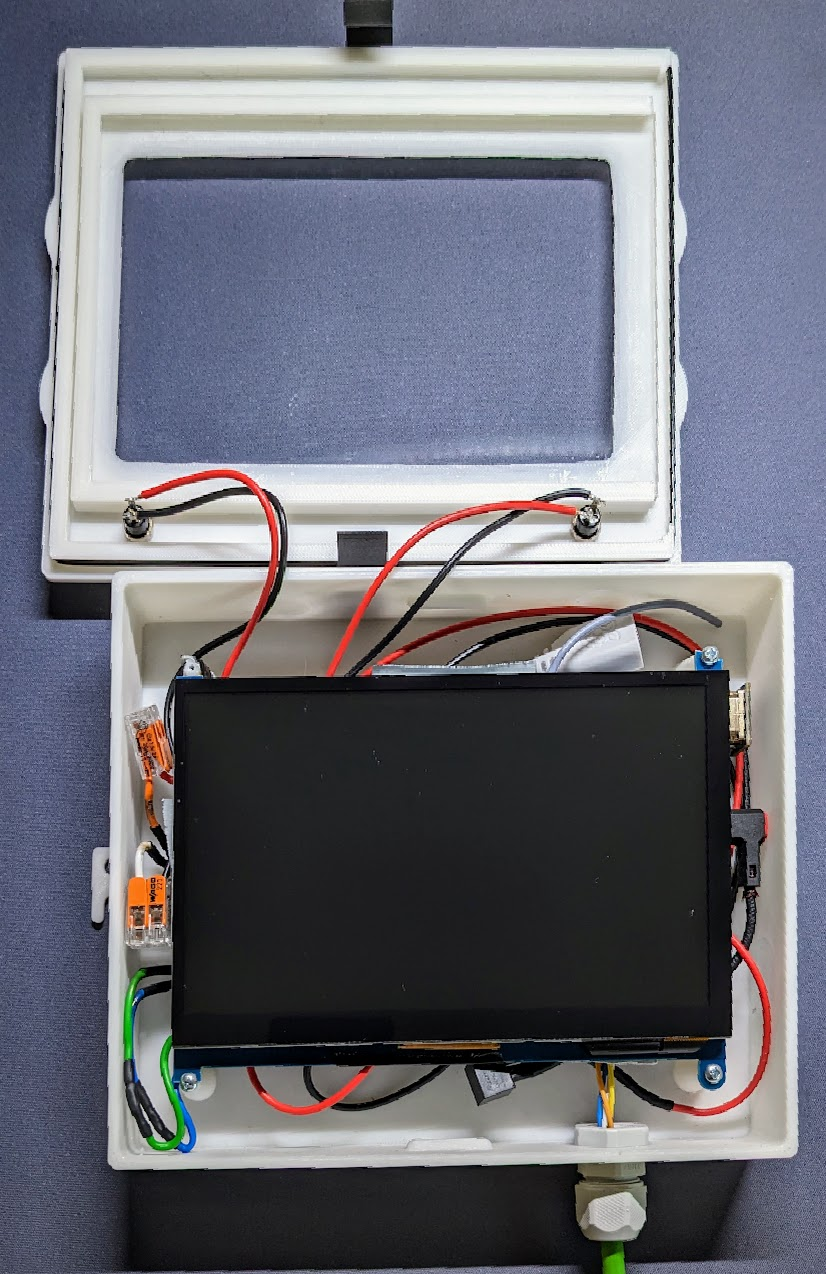
\includegraphics[width=0.99\textwidth]{prototyp_offen_w_display}
        \caption{Prototyp mit eingebautem Display \label{fig:prototyp_w_display}}
    \end{subfigure}
    \hfill
    \begin{subfigure}[r]{0.504\textwidth}
        \centering
        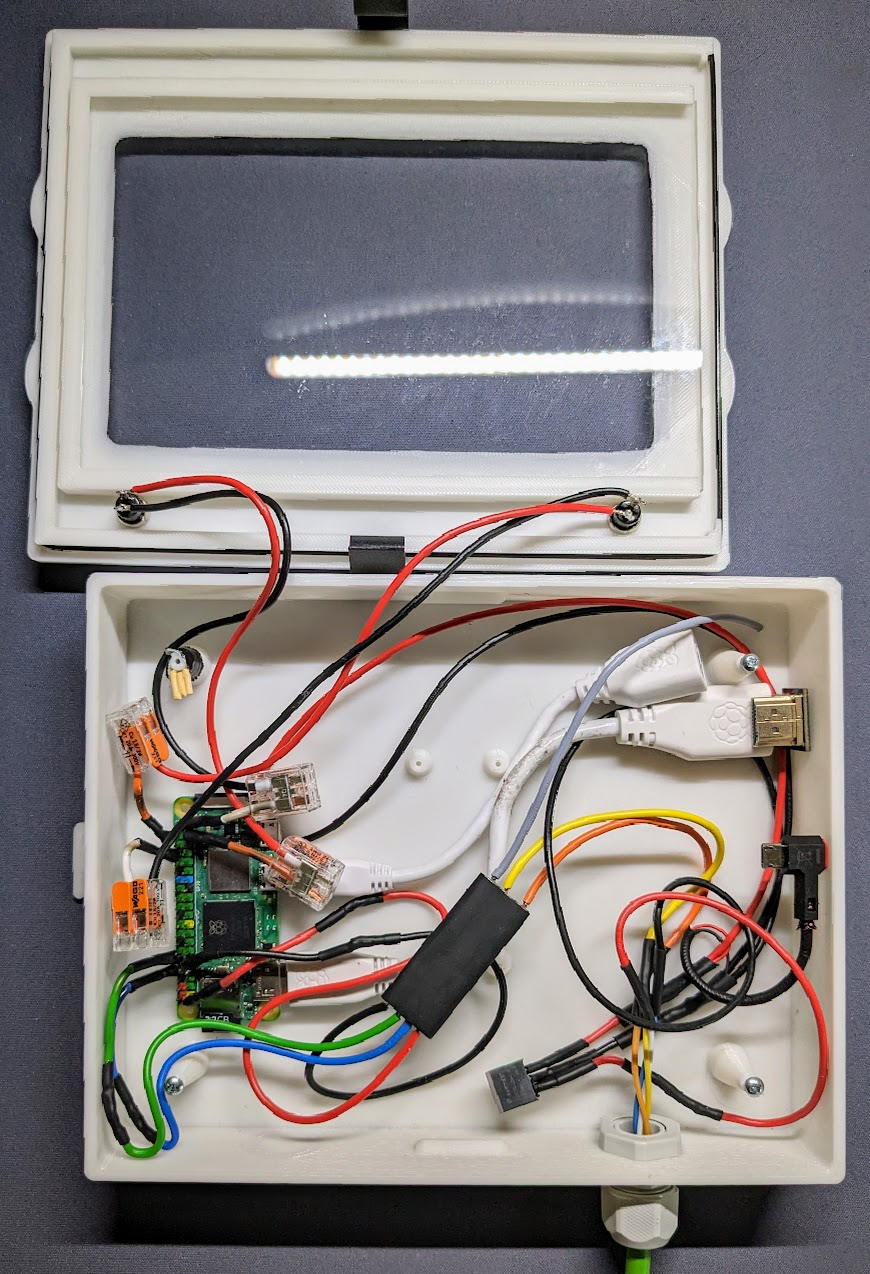
\includegraphics[width=0.99\textwidth]{prototyp_offen_w_o_display}
        \caption{Prototyp mit ausgebautem Display \label{fig:prototyp_w_o_display}}
    \end{subfigure}
	\caption{Prototyp der \ac{rltanzeige} von innen \label{fig:rlt_anzeige_prototyp}}
\end{figure}

Das Gehäuse des Prototyps ist 3D-gedruckt, um schnell Anpassungen machen zu können und nicht von einem vorgefertigten Gehäuse eingeschränkt zu werden. In diesem Gehäuse sind folgende Komponenten verbaut:

\begin{itemize}
    \item Der \textbf{Raspberry PI Zero 2 W} (siehe Abb.~\ref{fig:zero_2_w}) dient aufgrund seiner kleinen Größe und Rechenleistung als Rechner. Die Unterstützung von WLAN und Bluetooth lässt außerdem Raum zur Weiterentwicklung der \ac{rltanzeige}.
    \begin{figure}[H]
        \centering
        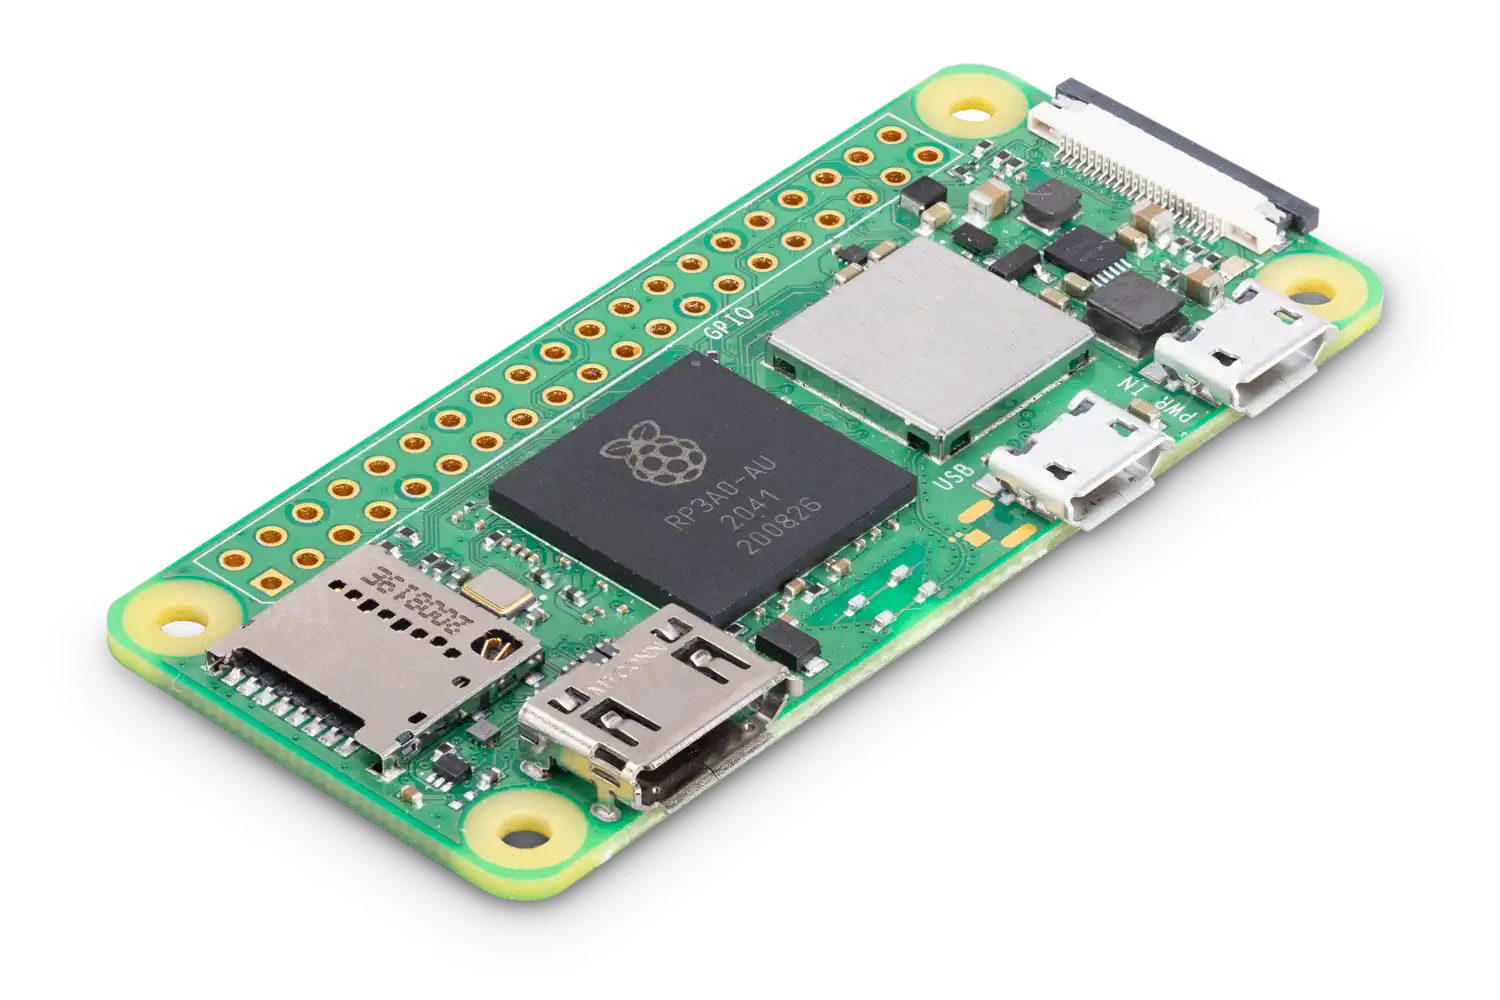
\includegraphics[width=7cm]{zero2-hero}
        \caption{Raspberry PI Zero 2 W (Quelle: \url{https://www.raspberrypi.com/products/raspberry-pi-zero-2-w/}) \label{fig:zero_2_w}}
    \end{figure}
    
    \item Das \textbf{7-Zoll Display} wird über \ac{hdmi} mit dem Raspberry PI verbunden und über Micro-USB mit Strom versorgt.

    \item Der \textbf{\ac{uart} zu \gls{gls_rs485} Adapter} (siehe Abb.~\ref{fig:ttl_rs485_adapter}) dient als Zwischenstück zwischen dem Raspberry PI und dem Bussystem. So kann das \gls{gls_rs485} Kabel mit den \ac{uart} Pins des Raspberry PIs verbunden werden.
    \begin{figure}[H]
        \centering
        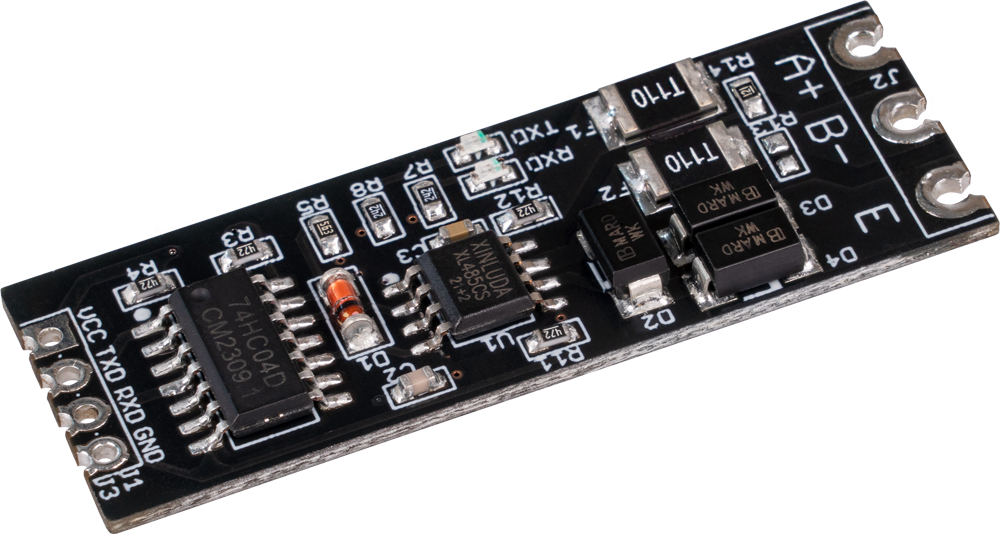
\includegraphics[width=6cm]{COM-TTL-RS4851}
        \caption{Joy-IT \ac{uart} TTL - \gls{gls_rs485} Konverter (Quelle: \url{https://joy-it.net/de/products/COM-TTL-RS485}) \label{fig:ttl_rs485_adapter}}
    \end{figure}

    \item Der \textbf{Spannungswandler} (siehe Abb.~\ref{fig:spannungswandler}) \bzw DC/DC Wandler wird benötigt, um die eingehende Spannung von 24 V auf 5 V zu reduzieren. Dabei werden sowohl der Raspberry PI als auch das Display von dieser Stromquelle versorgt.
    \begin{figure}[H]
        \centering
        
\includegraphics[width=5cm]{spannungswandler}
        \caption{Gaptec LME78\_05-1.0 DC/DC Wandler (Quelle: \url{https://www.conrad.de/de/p/gaptec-dc-dc-wandler-electronic-sip3-8-36vin-5vout-1000ma-11-6x8x10-4mm-856967933.html}) \label{fig:spannungswandler}}
    \end{figure}
\end{itemize}
\subsection{Erstellung des Raspberry PI \textit{Images}}
Technikerinnen und Techniker müssen die Schritte zum Aufsetzen eines Raspberry PIs (siehe Kapitel \ref{raspi_setup}) bei einer Neuinstallation nicht durchführen, da ihnen ein vorgefertigtes \gls{image} verabreicht wird. Dieses muss lediglich auf die SD-Karte des Raspberry PIs kopiert und nicht weiter konfiguriert werden. Die Erstellung dieses \gls{image}\textit{s} wird folgend erläutert. Das \gls{image} wird über ein Gerät mit Linux erstellt, daher kommt eine \ac{vm} zum Einsatz, um einfach eine Linux Distribution auf einem Windows Gerät laufen zu lassen. Dabei können unterschiedliche Linux Distributionen verwendet werden, wobei mindestens $4$ Gigabyte Arbeitsspeicher, $2$ Prozessorkerne und $80$ Gigabyte Festplattenspeicher empfohlen werden. 

\paragraph{\textit{Image} klonen}
Das \gls{image} wird erstellt, indem ein Speicherabbild einer SD-Karte mit funktionierendem Betriebssystem und Python Programm gemacht wird. Dieser Prozess findet hauptsächlich in der Kommandozeile statt, daher muss das Linux-Terminal geöffnet werden, um die folgenden Befehle auszuführen:
\begin{enumerate}
    %\item Zur Vorbereitung wird GParted mit \mintinline{console}{sudo apt-get install gparted} installiert. 

    \item Um die SD-Karte zu klonen, muss zuerst ihr Pfad mithilfe des Befehls \mintinline{console}{sudo fdisk -l} ermittelt werden. Dabei ist in Abb. \ref{fig:sudo_fdisk} zu sehen, dass der Pfad in diesem Beispiel \enquote{dev/sdb} ist.
    \begin{figure}[H]
        \centering
        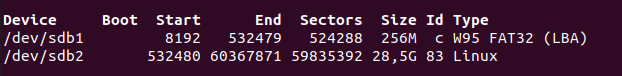
\includegraphics[width=0.75\linewidth]{sudo_fdisk}
        \caption{Ergebnis des \mintinline{console}{sudo fdisk -l} Befehls im Linux Terminal}
        \label{fig:sudo_fdisk}
    \end{figure}
    
    \item Im nächsten Schritt kann die SD-Karte geklont werden. Dazu wird der Befehl \mintinline{console}{dd} verwendet, wobei bei \mintinline{console}{if=} das input file \bzw der Pfad der SD-Karte angegeben wird und bei \mintinline{console}{of=} das output file \bzw der Pfad der \gls{image} (\enquote{.img}) Datei angegeben wird:
    \begin{minted}{console}
sudo dd if=/dev/sdb of=/home/ubuntu/Desktop/clone.img
    \end{minted}

    \item Da die aus dem vorgehenden Befehl generierte \gls{image} Datei mehr als $30$ Gigabyte groß ist, kann das \enquote{PyShrink} Skript verwendet werden, um das große  \gls{image} auf etwa $5$ bis $6$ Gigabyte zu verkleinern. \enquote{PyShrink} wird mit den folgenden Befehlen über die Kommandozeile installiert:
    \begin{minted}[breaklines=true, breakanywhere=true]{console}
wget https://raw.githubusercontent.com/Drewsif/PiShrink/master/pishrink.sh
chmod +x pishrink.sh
sudo mv pishrink.sh /usr/local/bin
    \end{minted}

    Nach der Installation, kann das \gls{image} mithilfe des nachfolgenden Befehls verkleinert werden. Hier wird ebenfalls zuerst der Pfad der Eingabedatei und dann der Pfad der Ausgabedatei angegeben:
    \begin{minted}[breaklines=true, breakanywhere=true]{console}
sudo pishrink.sh /home/ubuntu/Desktop/clone.img /home/ubuntu/Desktop/shrunken-image.img
    \end{minted}

    \item Das verkleinerte Image kann nun auf eine neue SD-Karte geflasht werden. Dafür kann ein beliebiger Imager, wie \zB \enquote{balenaEtcher} \enquote{Win32DiskImager} oder \enquote{RaspberryPi-Imager}, genutzt werden.
\end{enumerate}




